\documentclass[11pt]{article}

\usepackage[utf8]{inputenc}
\usepackage{amsmath}
\usepackage{amssymb}
\usepackage{cleveref}
\usepackage[T1]{fontenc}
\usepackage{fullpage}
\usepackage{graphicx}
\usepackage{mathbbol}
\usepackage{mathtools}
\usepackage{prftree}
\usepackage{stackrel}
\usepackage{stmaryrd}
\usepackage{url}
\usepackage{xspace}

%%% Theorem-like environments
\newtheorem{theorem}{Theorem}
\newtheorem{definition}{Definition}

%%% If using IEEEtrans
%%% \usepackage{cite}
%%% \interdisplaylinepenalty=2500

%%% If using article
\usepackage{cite}
\allowdisplaybreaks

%%% Generic

\newcommand{\df}{\emph}
\newcommand{\Rnum}[1]{\MakeUppercase{\romannumeral #1}}
\newcommand{\rnum}[1]{{\romannumeral #1}}
\newcommand{\NN}{\mathbb{N}}
\newcommand{\NNp}{\mathbb{N^+}}
\newcommand{\pr}[1]{\left\langle#1\right\rangle}
\newcommand{\Slash}{/\!/\xspace}
\newcommand{\pset}[1]{\mathcal{P}(#1)}
\newcommand{\code}[1]{\textsf{\small{#1}}}
\newcommand{\pto}{\rightharpoonup}
\newcommand{\Cpp}{C\textsuperscript{++}\xspace}
% xleftrightarrows, requires "stackrel".
\newcommand{\leftrarrows}{\mathrel{\raise.75ex\hbox{\oalign{%
  $\scriptstyle\leftarrow$\cr
  \vrule width0pt height.5ex$\hfil\scriptstyle\relbar$\cr}}}}
\newcommand{\lrightarrows}{\mathrel{\raise.75ex\hbox{\oalign{%
  $\scriptstyle\relbar$\hfil\cr
  $\scriptstyle\vrule width0pt height.5ex\smash\rightarrow$\cr}}}}
\newcommand{\Rrelbar}{\mathrel{\raise.75ex\hbox{\oalign{%
  $\scriptstyle\relbar$\cr
  \vrule width0pt height.5ex$\scriptstyle\relbar$}}}}
\newcommand{\longleftrightarrows}{\leftrarrows\joinrel\Rrelbar\joinrel\lrightarrows}
\makeatletter
\def\leftrightarrowsfill@{\arrowfill@\leftrarrows\Rrelbar\lrightarrows}
\newcommand{\xleftrightarrows}[2][]{\ext@arrow 
3399\leftrightarrowsfill@{#1}{#2}}
\makeatother
\newcommand{\abs}[1]{|#1|}

%%% matching logic related
\newcommand{\SV}{SV}
\newcommand{\EV}{EV}
\newcommand{\sig}{\mathbb{\Sigma}}
\newcommand{\app}{\mathit{app}}
\newcommand{\imp}{\to}
\newcommand{\dimp}{\rightleftarrows}
\newcommand{\cln}{{:}}
\newcommand{\ld}{\,.\,}
\newcommand{\Pattern}{\textsc{Pattern}}
\newcommand{\ip}[2]{[\![#1]\!]_{#2}}
\newcommand{\prule}[1]{(\textsc{#1})\xspace}
\newcommand{\appM}{\app_M}
\newcommand{\appMM}{\overline{\appM}}
\newcommand{\lfp}{{\mathbf{lfp}\,}}
\newcommand{\FV}{\mathit{FV}}
\newcommand{\inh}[1]{\llbracket #1 \rrbracket}

%%% K related
\newcommand{\K}{$\mathbb{K}$\xspace}
\newcommand{\cell}[2][]{\pr{#2}_{\code{#1}}}



\usepackage{color}
\usepackage{pifont}

\newcommand{\PS}{\mathcal{H}}
\newcommand{\oldPS}{\mathcal{P}}
\newcommand{\lam}{\mathsf{lambda}}
\newcommand{\intt}{\mathit{intension}}
\newcommand{\Var}{\mathit{Var}}
\newcommand{\always}{\square}
\newcommand{\until}{\mathbin{U}}
\newcommand{\eventually}{\diamond}
\newcommand{\To}{\Rightarrow}
\newcommand{\lsegleft}{\mathit{ll}}
\newcommand{\sand}{\mathbin{*}}
\newcommand{\lst}{\mathit{list}}
\newcommand{\hole}{\square}
\newcommand{\ic}[2]{#1 -o #2}
\newcommand{\varphipre}{\varphi_\mathit{pre}}
\newcommand{\varphipost}{\varphi_\mathit{post}}
\newcommand{\onenext}{\bullet}
\newcommand{\allnext}{\circ}
\newcommand{\BETA}{\prule{$\beta$}}
\newcommand{\intension}{\mathsf{intension}}
\newcommand{\vDashH}{\vDash_H}
\newcommand{\DD}{\mathcal{D}}
\newcommand{\cev}{\mathsf{ev}}
\newcommand{\csv}{\mathsf{sv}}
\newcommand{\csymb}{\mathsf{symbol}}
\newcommand{\cprop}{\mathsf{prop}}
\newcommand{\cex}{\mathsf{exists}}
\newcommand{\cmu}{\mathsf{mu}}
\newcommand{\cfull}{\mathsf{full}}
\newcommand{\capp}{\mathsf{app}}
\newcommand{\fl}{\rightsquigarrow}
\newcommand{\Gapa}{\Gamma_{\overline{\app},1}}
\newcommand{\Gapb}{\Gamma_{\overline{\app},2}}
\newcommand{\Wit}{\mathit{Wit}}
\newcommand{\emp}{\mathit{emp}}
\newcommand{\simp}{\mathbin{-\!*}}
\newcommand{\nil}{\mathit{nil}}
\newcommand{\empheap}{\bot_\mathit{heap}}
\newcommand{\vDashSL}{\vDash_\mathsf{SL}}
\newcommand{\Map}{\mathit{Map}}
\newcommand{\Nat}{\mathit{Nat}}
\newcommand{\suc}{\mathit{succ}}
\newcommand{\zero}{\mathit{zero}}
\newcommand{\SL}{\mathsf{SL}}
\newcommand{\obj}{\mathsf{obj}}
\newcommand{\PC}{\mathsf{ProofCheck}}
\newcommand{\mlmm}{\textsf{ml.mm}\xspace}
\newcommand{\cmark}{{\color{darkcyan}\ding{51}}}
\newcommand{\xmark}{{\color{red}\ding{55}}}
\newcommand{\qmark}{\textbf{?}}
\definecolor{darkcyan}{rgb}{0.0, 0.55, 0.55}
\newcommand{\cmarkx}
{{\color{darkcyan}\ding{51}\textsuperscript{\kern-0.55em\tiny\ding{55}}}}
\newcommand{\plan}[1]{{\color{darkcyan}#1}}
\newcommand{\InitState}{\mathit{InitState}}


\title{A Practical Trustworthy Language Framework\\ \large Thesis 
Proposal}
\author{Xiaohong Chen \\ University of Illinois at Urbana-Champaign \\ 
\url{xc3@illinois.edu}}
\date{}

\begin{document}

\maketitle

\tableofcontents

\section{Introduction}

A \emph{language framework} is an artifact that allows language designers to 
define the formal syntax and semantics of their programming 
languages using an intuitive and easy-to-understand meta-language. 
Once the formal syntax and semantics definition is given, the framework automatically generates all language tools of that language from 
its formal definition in a correct-by-construction manner, at no additional 
costs. 
By language tools, I mean both an \emph{implementation} of the language
that often consists of a parser and an interpreter and/or a compiler
so as to execute programs written in that language
and \emph{formal analysis tools} such as a deductive program verifier
and a bounded model checker. 
The above is called the \emph{vision of an ideal language framework},
illustrated in \Cref{fig:ideal}. 

\begin{figure}
\centering
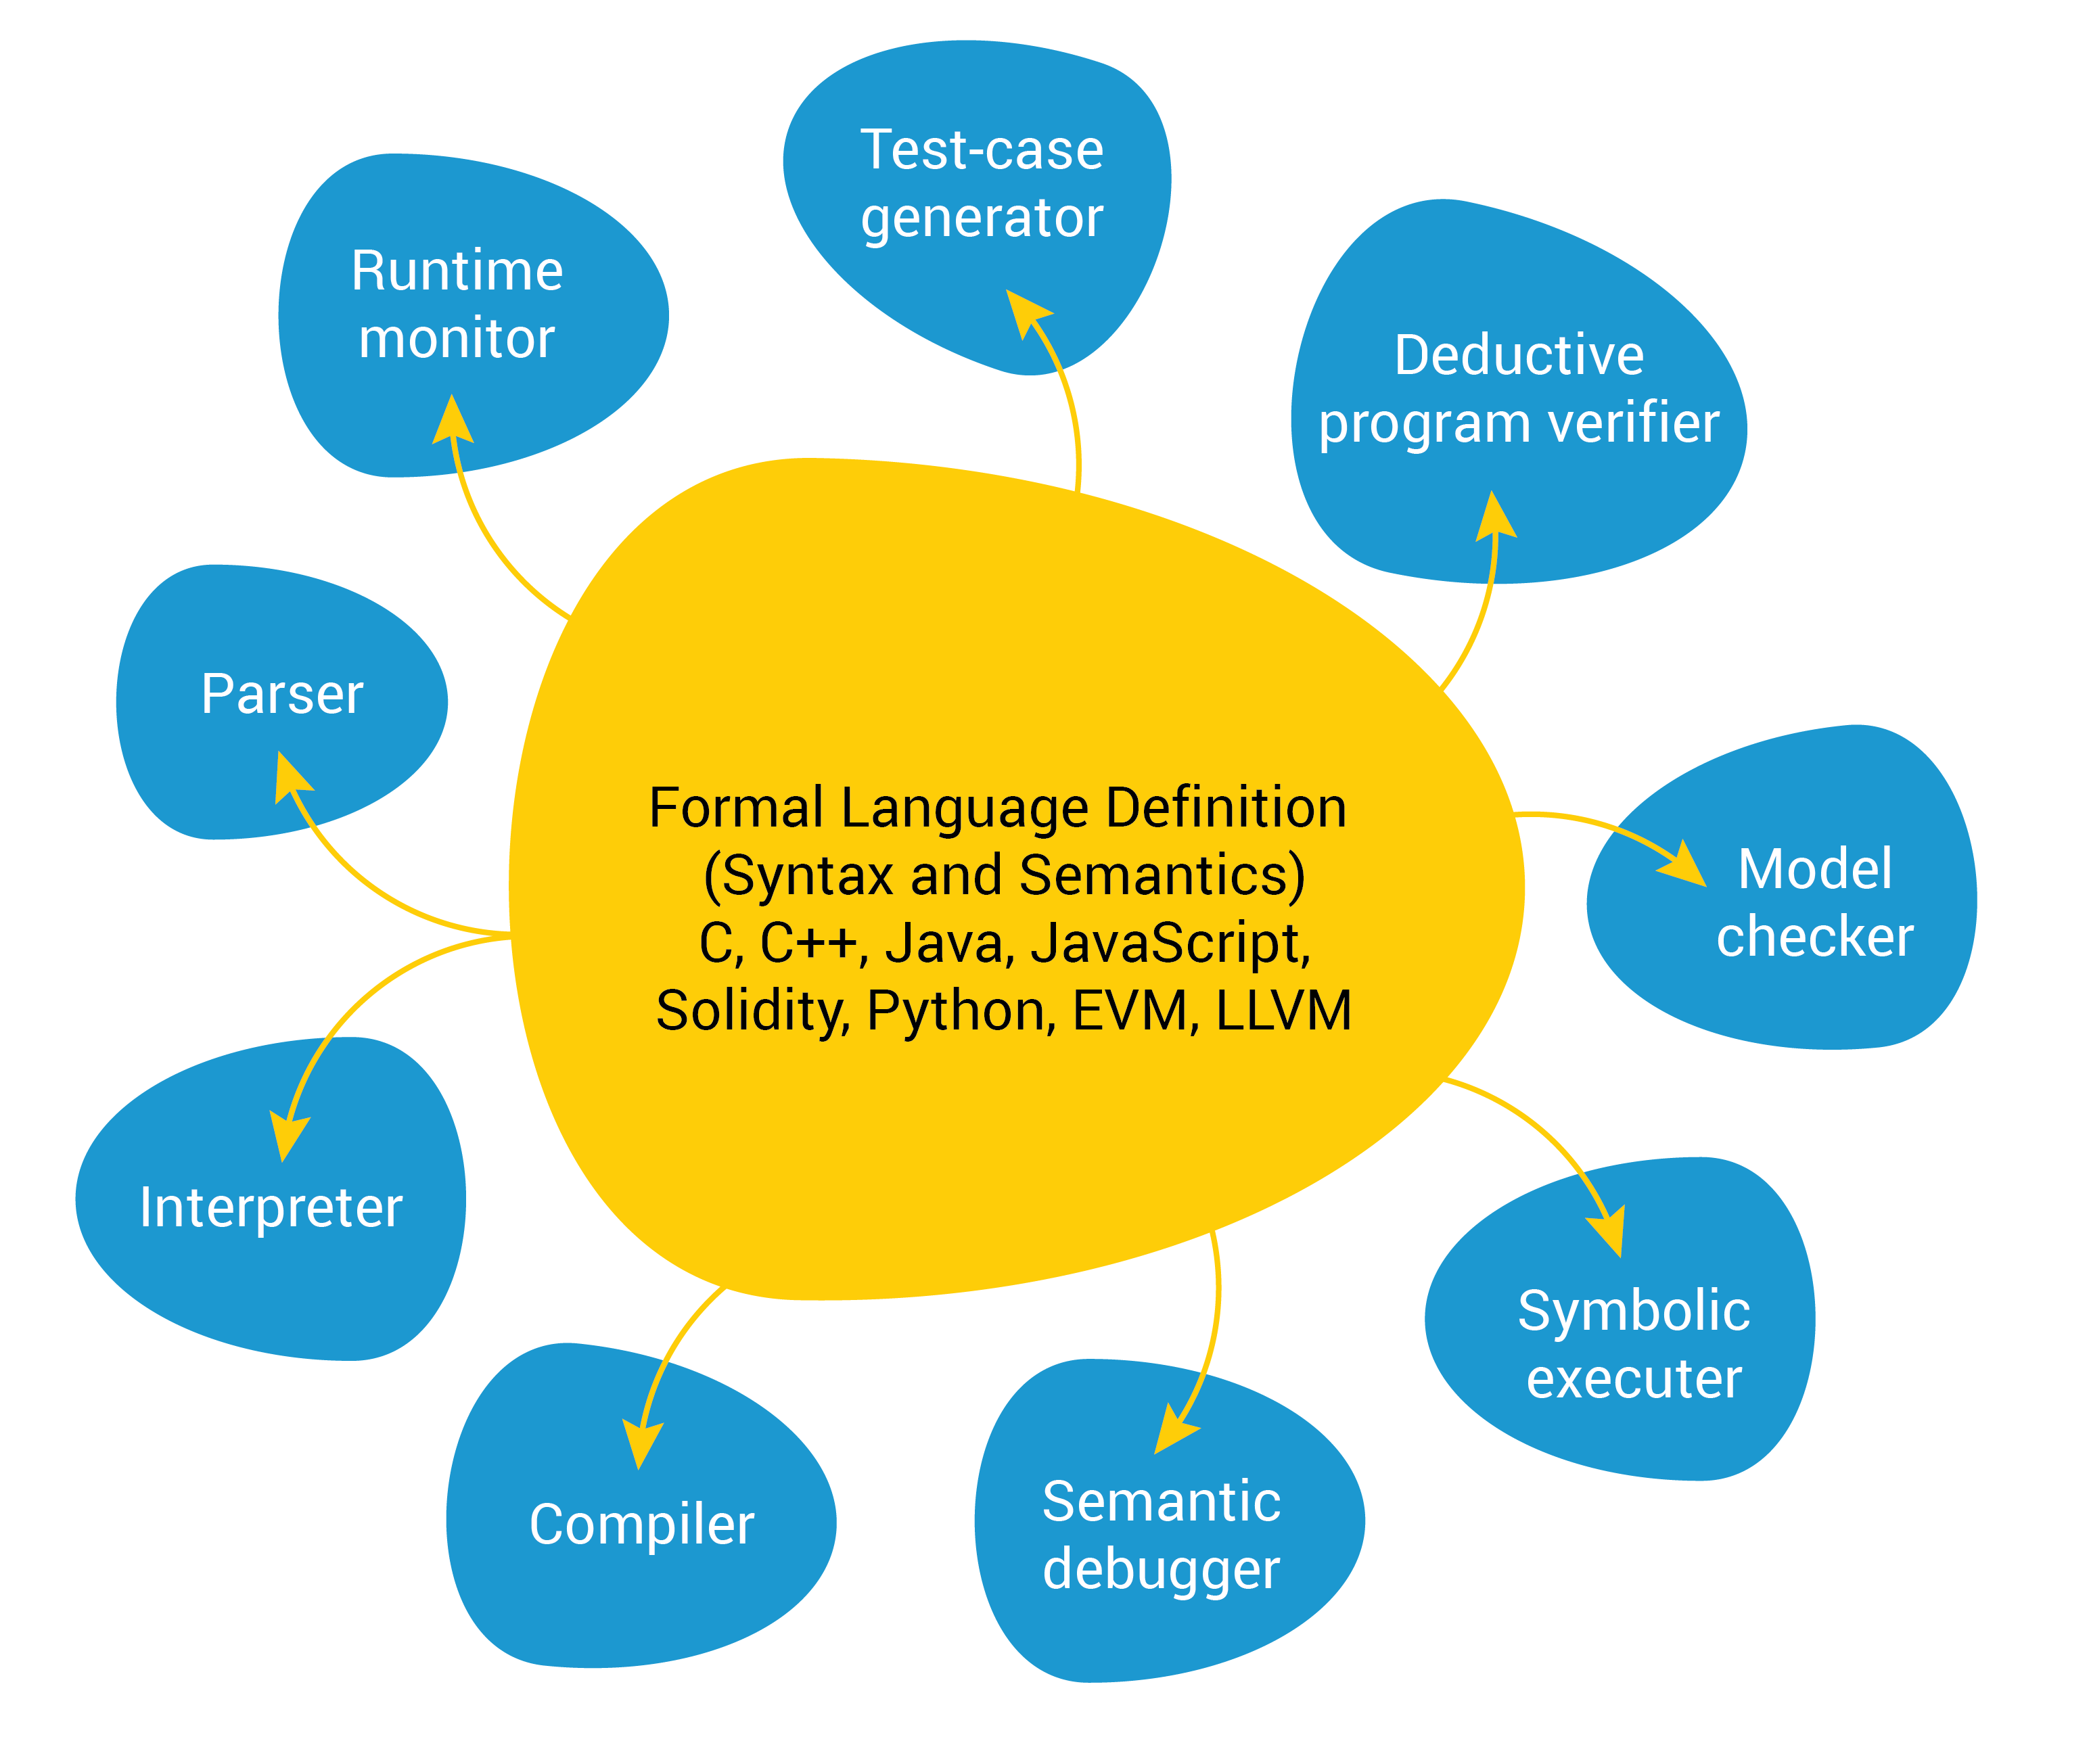
\includegraphics[width=0.6\columnwidth]{figs/k-vision.png}
\caption{Vision of an ideal language framework.}
\label{fig:ideal}
\end{figure}

The \K language framework (\url{http://kframework.org}) is a pursuer of the 
above ideal vision and has achieved much success in practice.
Using \K, the formal definitions of many real-world languages
have been defined and their implementations and formal analysis tools have been 
automatically generated. 
As of this writing, \K has successfully been used to define the following 
programming languages:
C \cite{HER15},
Java \cite{BR15},
JavaScript \cite{PSR15},
Python \cite{Gut13},
Ethereum virtual machine bytecode \cite{HSZ+18},
x86-64 \cite{DPK+19}
and to generate their language tools. 
There are commercial products based on the tools generated by \K
(\url{https://runtimeverification.com/}). 

\K has had several different implementations, all of which are complex. 
The most recent \K implementation (\url{https://github.com/kframework/k})
is developed in several languages including
Haskell, \Cpp, Scala, and OCaml, with more than 500,000 lines of code.
It consists of a front end that compiles a language definition written in \K
using an intuitive and compact human-readable meta-language into 
one that is written in a lower level language (called Kore) where 
syntactic sugar, user-defined notations, comments, shortcuts, and other
front end syntax are eliminated.
The resulting lower-level Kore definition is not as human-readable as the original \K 
definition but it can be easily understood and processed by \K's back ends.
These back ends implement complex algorithms to generate the language tools
and to conduct various tasks such as program execution, formal verification, and 
symbolic execution. 

A serious question is how to guarantee the \emph{correctness}
of a language framework implementation, such as \K,  which has a large code 
base and implements complicated algorithms.
In other words, if we define a programming language in \K and
use \K to execute a program written in that language, 
to what extend can we trust the execution result that \K returns?
Similar questions can be asked not only for program execution but also for
formal verification, symbolic execution, bounded model checking, 
and many other formal analysis tools that \K generates for the language.
In short, what is the trust base of \K?

Currently, to trust the execution result that \K returns
(or any other execution and/or analysis tasks that \K conducts)
%or any concrete tasks that \K does such as symbolically executing a program for 
%a given number of steps
%or verifying a function property of a program, 
we need to trust the entire code base of \K, which is large and certainly contains bugs.
My research goal is to make that trust base smaller, from more than
500,000 lines of code written in four different programming languages,
to a small \emph{proof checker}
\cite{ml-checker}
that has only 245 lines of code, \emph{without} the need to re-implement the 
existing \K
front and back ends. 
This way, I make \K a \emph{trustworthy} and \emph{practical} language 
framework.

In this proposal, I discuss the methodology to accomplish the above goal. 
I first give an overview of the proposed method in \Cref{sec:method}.
Then I discuss the work that has been done in \Cref{sec:current}
and the proposed future work in \Cref{sec:proposed}. 
%I give a 12-month timeline to finish the proposed future work in 
%\Cref{sec:timeline}.
A timeline to finish the proposed work in 12 months is given at the end of \Cref{sec:method}. 

\section{Overview of Proposed Method}
\label{sec:method}

The proposed method is based on a \emph{logical foundation} of \K.

In short, I design a mathematical logic called \emph{matching logic} that aims 
at serving as the logical foundation of \K. 
By that, I mean that each \K definition of a programming language $L$
yields a \emph{matching logic theory} $\Gamma^L$ that includes the definition
of
the syntax and semantics of $L$. 
Further, each task that \K does for the language $L$ 
is expressed by a matching logic formula $\varphi$, called a \emph{pattern}. 
For example, the task where we use \K to run the following C program snippet
$$
\code{SUM} \equiv \code{while(!n) \{ s=s+n; n=n-1; \} }
$$
on a state where \code{n} is 100 and \code{s} is 0,
and that \K returns the value 5050, can be expressed by the 
following 
matching logic pattern, intuitively:
{\allowdisplaybreaks[0]\begin{align}
\Gamma^\textrm{C} \vdash
& \cell[cfg]{\cell[code]{\code{SUM}} \cell[state]{\code{n}\mapsto 100, 
\code{s}\mapsto 0}} \To^*
\cell[cfg]{\cell[code]{\code{.}} \cell[state]{\code{n}\mapsto 0, 
\code{s}\mapsto 5050}}
\label{eq:po-exe-sum}
\end{align}}%
where $\Gamma^\textrm{C}$ is a matching logic theory that includes the formal 
syntax and semantics of C
and $\cell[cfg]{\cell[code]{c} \cell[state]{\rho}}$
is the (matching logic) pattern that represents a computation configuration\footnote{The actual computation configurations for C are more complicated, with more than a hundred \emph{configuration cells} that 
hold the necessary semantic information needed for program execution.
Here, we simplify it into a configuration with only two cells 
(\code{code} that holds the computation and \code{state} that holds the program state) for the sake of presentation.}
where the current code is $c$ and the program state is $\rho$. 
The symbol ``$\To^*$'' specifies the rewriting/reachability relation
between the two configurations, meaning that the first configuration
eventually reaches the second configuration within finitely many execution steps (\Cref{sec:ml-expressiveness}).
Its semantics is defined by the matching logic theory $\Gamma^\textrm{C}$ using
patterns/axioms.
%Besides program execution, other formal 
%Tasks other than program execution are expressed by the corresponding matching 
%logic patterns, too. 

The key idea to achieve a small trust base for \K is as follows. 
We encode the correctness of \K conducting a task,
say executing the above C program \code{SUM} and returning the value 5050 using C semantics, 
into a \emph{matching logic formal proof}
$\Gamma^\textrm{C} \vdash \varphi$ like \Cref{eq:po-exe-sum},
which derives $\varphi$ from $\Gamma^L$ using one fixed 
\emph{matching logic proof system} (\Cref{fig:ps}). 
The formal proof $\Gamma^\textrm{C} \vdash \varphi$ is further encoded into a 
\emph{proof object} that is annotated with the detailed proof steps,
so the proof object witnesses the formal proof
and can be quickly checked by a \emph{matching logic proof checker},
which implements the proof rules in the proof system in \Cref{fig:ps}.
This way, the correctness of \K conducting one task is reduced to
the correctness of the proof checker checking one proof object.
This is preferable,
because the proof checker is much smaller than the 
entire \K implementations. 
I implemented a prototype proof checker in \cite{ml-checker} using the Metamath language \cite{metamath} in 245 lines of code.

The key observation is that
correctness is established for each individual task that \K does 
on a \emph{case-by-case} basis, and not for the entire \K code base. 
If the bugs in \K are not triggered when \K conducts the task, the correctness 
is not compromised and a proof object can be generated. 
If the bugs are triggered, the correctness is lost and there does 
not exist a corresponding proof object for the wrong result that \K 
returns.
Therefore, proof objects serve as \emph{correctness certificates}
that need to be issued for each tasks that \K carries out. 

The above proposed approach can be broke down into the following deliverables:
\begin{enumerate}
\item a proposal of the logical foundation---matching logic---of \K; this should include the syntax, the semantics, and the proof system of matching logic;
\item a collection of matching logic theories that define the common logical 
systems that are used to specify the formal semantics of programming 
languages and program properties; this guarantees that matching logic 
has the expressiveness that is needed to encode tasks that a language framework 
should usually support;
\item a completeness result of matching logic proof system;
this establishes the connection between matching logic semantics and its formal 
deduction so that we know the proof rules proposed in item 1 are not ad-hoc;
\item decidable fragment of matching logic and their corresponding decision procedures; this brings up the level of automation in the current \K implementations;
\item a matching logic proof checker that is small and fast and a proof object generator that encodes the tasks that \K conducts such as program execution and formal verification into proof objects that can be proof-checked by the proof checker.
\end{enumerate}


\paragraph{Publications and timeline.}

The deliverables that have been finished are discussed in \Cref{sec:current}
and those that are planned for the future are discussed in 
\Cref{sec:proposed}. 
I summarize them in the following.
For each item, I associate the corresponding publications (in \textbf{black}) 
as well as the planned submissions (in \textbf{\plan{green}}).

\begin{itemize}
\item Current results that have been published include:
\begin{enumerate}
\item \textbf{\cite[LICS2019]{CR19}}: the proposal of matching logic and a 13-rule Hilbert-style proof system 
(\Cref{sec:ml} and \Cref{fig:ps});
\item results showing that many important logical systems can be defined as matching logic theories (\Cref{sec:ml-expressiveness} and \Cref{fig:logics}), including
\begin{enumerate}
\item \textbf{\cite[LICS2019]{CR19}}: FOL, FOL with least fixpoints, modal logic, temporal logics, dynamic logic, modal $\mu$-calculus, and reachability logic;
\item \textbf{\cite[ICFP2020]{CR20}}: $\lambda$-calculus, $\pi$-calculus, and type systems;
\item \textbf{\cite[TechRep2020]{CLR20}}: initial algebra semantics, planned for \textbf{\plan{[LICS2021]}};
\end{enumerate}
\item \textbf{\cite[OOPSLA2020]{CTR20}}: 
a prototype  automated theorem prover of matching logic, focusing on fixpoitn reasoning (\Cref{sec:mlprover});
\item \textbf{\cite[LICS2019]{CR19}}: some preliminary completeness results (\Cref{sec:known-complete}).
\end{enumerate}
\item Future work (including work that has partial results) includes:
\begin{enumerate}
\item a matching logic proof checker and a procedure to generate proof objects (\Cref{sec:proposed-mlpc}), where
\begin{enumerate}
\item an prototype proof checker implemented in Metamath and the proof object generation for a simple imperative language are planned for \textbf{\plan{[CAV2021]}};
\item a full integration of proof object generation for program execution and formal verification into \K is planned for \textbf{\plan{[PLDI2022]}};
\end{enumerate}
\item a completeness theorem based on Henkin semantics (\Cref{sec:proposed-complete}), planned for \textbf{[\plan{LICS2021}]};
\item decidable fragments of matching logic and their decision procedures 
(\Cref{sec:proposed-decision}), planned for \textbf{[\plan{LICS2021}]};
\item matching logic theories that define separation logic and hyper linear 
temporal logic (\Cref{sec:proposed-logics}), planned for \textbf{[\plan{POPL2022}]} and \textbf{[\plan{LICS2021}]}, respectively.
\end{enumerate}
\end{itemize}

\section{Current Results}
\label{sec:current}

In this section, I summarize the main research results obtained so far. 

\subsection{Proposal of Matching Logic}
\label{sec:ml}

I proposed with my supervisor professor Grigore Ro\c{s}u \emph{matching logic}
in its full generality \cite{CR19}. 
Matching logic serves as the unifying logical foundation of the proposed 
trustworthy language framework. 
Its syntax is parametric in a \emph{signature} that consists of 
user-provided \emph{symbols} and defines formulas, called \emph{patterns}, to 
uniformly represent
data structures, mathematical objects, computations, program configurations,
transition relations, dynamic properties of programs, and so on. 
Its semantics defines \emph{models}, which can be constrained by
a set of user-provided \emph{pattern axioms}. 
A matching logic \emph{proof system} is used to derive new patterns from a 
given set of axioms. 

The power of matching logic lies in its simplicity and expressiveness. 
In terms of simplicity, matching logic follows a minimalism design. 
For example, the syntax of matching logic patterns, shown below, has only 8 
syntactic constructs that define the most
basic concepts that are necessary to serve as the logical foundation of a 
language framework:
\begin{align*}
\varphi &\Coloneqq x &&\text{\Slash element variables} \\
&\ \ \mid X && \text{\Slash set variables} \\
&\ \ \mid \sigma && \text{\Slash symbols (from a user-provided signature)} \\
&\ \ \mid \varphi_1 \, \varphi_2 && \text{\Slash application} \\
&\ \ \mid \bot && \text{\Slash bottom} \\
&\ \ \mid \varphi_1 \imp \varphi_2 && \text{\Slash implication} \\
&\ \ \mid \exists x \ld \varphi && \text{\Slash quantification} \\
&\ \ \mid \mu X \ld \varphi && \text{\Slash least fixpoints}
\end{align*}
Every syntactic construct in the above has a unique purpose, which I explain 
intuitively. 
Element variables are used to refer to the individual elements in the models,
like FOL variables.
Set variables are used to refer to the sets of elements in the models, like 
propositional variables in modal logic. 
Symbols are provided by the users and are used to represent constructors, 
functions, predicates, relations, and so on, whose actual semantics is 
determined by the axioms and theories. 
An application construct is used to apply a symbol (or any pattern in general)
to an argument pattern. 
Bottom and implication allow us to build logical constraints. 
Quantification allows us to create abstraction.
Least fixpoints allow us to define induction and recursion. 

Besides the syntax, matching logic has a 13-rule Hilbert-style proof system
(\Cref{fig:ps}) that derives proof judgments of the form
$\Gamma \vdash \varphi$, meaning that $\varphi$ can be proved using the proof 
system from the axioms in $\Gamma$. 

\begin{figure}[t]
{\centering\small
\hspace*{-6ex}
$
\begin{array}{l}
  \begin{array}{l} \textrm{FOL} \\ \textrm{Reasoning} \end{array} 
  \left \{ \begin{array}{l} \\[20ex] \end{array}\right.
\\
  \begin{array}{l} \textrm{Frame} \\ \textrm{Reasoning} \end{array} 
  \left \{ \begin{array}{l} \\[16ex] \end{array}\right.
\\
  \begin{array}{l} \textrm{Fixpoint} \\ \textrm{Reasoning} \end{array} 
  \left \{ \begin{array}{l} \\[13ex] \end{array}\right.
\\
  \begin{array}{l} \textrm{Technical} \\ \textrm{Rules\ \ \ \ \  \ } 
  \end{array} 
  \left \{ \begin{array}{l} \\[6ex] \end{array}\right.
\end{array}$\hspace*{-1ex}
\begin{tabular}{ll}
\hline\\[-2.5ex]
\prule{Tautology} &
$\varphi$ \quad
if $\varphi$ is a tautology
 \\[0.3ex]
\prule{Modus Ponens} &
$
\begin{prftree}
{\varphi_1}{\varphi_1 \imp \varphi_2}
{\varphi_2}
\end{prftree}$
\\[0.3ex]
\prule{$\exists$-Quantifier} &
$\varphi[y/x] \imp \exists x \ld \varphi$
\\[1.2ex]
\prule{$\exists$-Generalization} &
$
\begin{prftree}[r]{if $x \not\in \FV(\varphi_2)$}
{\varphi_1 \imp \varphi_2}
{(\exists x . \varphi_1) \imp \varphi_2}
\end{prftree}
$
\\[1.2ex]\hline\\[-2.5ex]
\prule{Propagation$_\bot$} &
$C[\bot] \imp \bot$
\\[1.2ex]
\prule{Propagation$_\vee$} &
$C[\varphi_1 \vee \varphi_2] \imp 
C[\varphi_1] \vee C[\varphi_2]$
\\[1.2ex]
\prule{Propagation$_\exists$} &
$C[\exists x \ld \varphi]
 \imp \exists x \ld C[\varphi]$ \ \ 
if $x \not\in \FV(C)$
\\[1.2ex]
\prule{Framing} &
$
\prftree{\varphi_1 \imp \varphi_2}
{C[\varphi_1]  \imp C[\varphi_2]}
$
\\[.5ex]\hline\\[-2.8ex]
\prule{Substitution} &
$\prftree{\varphi}{\varphi[\psi/X]}$
\\[1.2ex]
\prule{PreFixpoint} &
${\varphi [(\mu X \ld \varphi) / X] \imp \mu X \ld \varphi}
$
\\[1.2ex]
\prule{Knaster-Tarski} &
$\prftree{\varphi[\psi / X] \imp \psi}
{\mu X \ld \varphi \imp \psi}
$
\\[1.2ex]\hline\\[-2.5ex]
\prule{Existence} &
$\exists x \ld x$ 
\\[1.2ex]
\prule{Singleton} &
$\neg \, (C_1[x \wedge \varphi] \wedge C_2[x \wedge \neg \varphi])$
\\\hline
\end{tabular}
\\[1.5ex]
\qquad\qquad\qquad\qquad\qquad\qquad\quad
where $C[\varphi]$ denotes application $\varphi \, \psi$ or $\psi\, \varphi$ 
for any $\psi$.}
\caption{Matching logic has a Hilbert-style proof system with 13 
proof rules. }
\label{fig:ps}
\end{figure}

The simplicity of matching logic means that the more involved concepts such as 
sorts, many-sorted functions, many-sorted predicates, order-sorted structures,
subsort overloading, types, dependent types, parametric types, and so on
are not built into it.
Instead, they can be defined in an axiomatic way by matching 
logic theories using symbols and axioms. 
I explain it in \Cref{sec:ml-expressiveness}.

I emphasize the simplicity of matching logic because it makes 
\emph{proof checking} simple. 
A proof checker is a decision procedure whose input is 
a \emph{proof object} that encodes a formal proof $\Gamma \vdash \varphi$.
The proof checker checks whether the given proof object is valid. 
Thanks to the simplicity of matching logic syntax and its proof system,
a matching logic proof checker can be implemented in 245 LOC in 
Metamath \cite{ml-checker}.
In \Cref{sec:proposed-mlpc}, I explain how the proof checker serves as a small 
trust base of the proposed trustworthy language framework that
is accessible to the users. 

%Matching logic has a \emph{pattern matching semantic};
%therefore, a matching logic pattern $\varphi$ is not interpreted as true or 
%false as in first-order logic (FOL), but as a set, containing the elements 
%that 
%can \emph{match} it. 
%Formally, a matching logic \emph{model} is a nonempty set $M$ associated with
%\begin{enumerate}
%\item an application interpretation $\appM \colon M \times M \to 
%\pset{M}$, and
%\item a symbol interpretation $\sigma_M \subseteq M$ for each $\sigma \in 
%\Sigma$,
%\end{enumerate}
%where $\pset{M}$ is the power set of $M$. 
%Note that application is interpreted as a binary function that returns subsets 
%of $M$ and not elements in $M$. 
%Also, symbols are interpreted as subsets and not elements. 
%Given a \emph{variable valuation} $\rho$ such that
%\begin{enumerate}
%\item $\rho(x) \in M$ for all element variables $x$ and
%\item $\rho(X) \subseteq M$ for all set variables $X$,
%\end{enumerate}
%we define \emph{pattern interpretation}
%$\ip{\varphi}{M,\rho} \subseteq M$ inductively as follows:
%\begin{enumerate}
%\item $\ip{x}{M,\rho} = \{ \rho(x) \}$,
%\item $\ip{X}{M,\rho} = \rho(X)$,
%\item $\ip{\sigma}{M,\rho} = \sigma_M$,
%\item $\displaystyle \ip{\varphi_1 \, \varphi_2}{M,\rho} = 
%\appMM(\ip{\varphi_1}{M,\rho}
%\ip{\varphi_2}{M,\rho}) = \bigcup_{a_1 \in \ip{\varphi_1}{M,\rho}, a_2 \in 
%\ip{\varphi_2}{M,\rho}} \appM(a_1,a_2)$,
%\item $\ip{\bot}{M,\rho} = \emptyset$,
%\item $\ip{\varphi_1 \imp \varphi_2}{M,\rho} = M \setminus 
%(\ip{\varphi_1}{M,\rho} \setminus \ip{\varphi_2}{M,\rho})$,
%\item $\ip{\exists x \ld \varphi}{M,\rho} = \bigcup_{a \in M} 
%\ip{\varphi}{M,\rho[a/x]}$,
%\item $\ip{\mu X \ld \varphi}{M,\rho} = \lfp \lambda A \mapsto 
%\ip{\varphi}{M,\rho[A/X]}$, where $\lambda A \mapsto 
%\ip{\varphi}{M,\rho[A/X]}$ is the function that maps $A \subseteq M$ to  
%$\ip{\varphi}{M,\rho[A/X]}$, which we prove monotone. 
%\end{enumerate}


%In FOL, we build \emph{terms} to represent elements and \emph{formulas} to 
%state propositions. 
%In matching logic, terms and formulas are unified by patterns. 
%A term $t$ can be regarded as a pattern whose interpretation
%$\ip{t}{M,\rho}$ is always a singleton set. 
%A (FOL) formula $\psi$ can be regarded as a pattern whose interpretation
%$\ip{\psi}{M,\rho}$ is either the total set $M$, which represents ``true'',
%or the empty set $\emptyset$, which represents ``false''. 


%Matching logic allows users to define \emph{theories}.
%A matching logic theory $\Gamma$ consists of a set of patterns called 
%\emph{axioms}, which are used to constrain the models. 
%Formally speaking, given a theory $\Gamma$, we write $M \vDash \Gamma$ if all 
%axioms in $\Gamma$  are interpreted as the total set $M$, i.e., ``true''. 
%Therefore, matching logic can be used as a \emph{specification language}. 
%Indeed, let $M^*$ be an intended model that we want to specify.
%If there exists a theory $\Gamma^*$ such that
%for all $M \vDash \Gamma^*$, $M$ is isomorphic to $M^*$, then we say that
%$\Gamma^*$ captures precisely $M^*$. 

%Matching logic has a Hilbert-style proof system that defines the 
%\emph{provability relation} $\Gamma \vdash \varphi$, which means that 
%$\varphi$ 
%can be proved under theory $\Gamma$. 
%Let us also define the validity relation, written $\Gamma \vDash \varphi$, 
%to mean that for all $M \vDash \Gamma$ we have $M \vDash \varphi$.
%Then, the following soundness theorem is proved.
%\begin{theorem}[Soundness]
%\label{thm:soundness}
%$\Gamma \vdash \varphi$ implies $\Gamma \vDash \varphi$. 
%\end{theorem}

%The soundness theorem allows us to use matching logic as a \emph{formal 
%deduction system}.
%Indeed, if $M^*$ is the intended model and $\Gamma$ consists of \emph{some}
%patterns $\psi$ such that $M^* \vDash \psi$, then we can use the matching 
%logic 
%proof system to derive patterns that are provable within $\Gamma$. 
%If $\Gamma \vdash \varphi$, then by \Cref{thm:soundness}, $\Gamma \vDash 
%\varphi$, and since $M^* \vDash \varphi$ we have $M^* \vDash \varphi$. 
%Therefore, matching logic proof system allows us to formally prove patterns 
%$\varphi$ that hold in $M^*$. 
%This does not require $\Gamma$ to capture precisely $M^*$. 
%The more patterns $\Gamma$ has, the more patterns we can prove about $M^*$. 



%In terms of expressiveness, matching logic defines logical theories to capture 
%the formal deduction and/or models that are defined by other logical systems. 
%So far, many commonly used logical systems have been considered;
%these are shown in \Cref{fig:logics}.
%More logical systems will be considered as future work (\Cref{sec:proposed}). 



%To answer the second question: matching logic is simple. 
%It follows a minimalist design. 
%Its syntax has 8 syntactic constructs and its proof system has 15 proof rules
%(\Cref{fig:proof-rules}). 
%It only includes the most basic and necessary as the built-ins
%and leave the complex concepts such as equality, functions, predicates, sorts, 
%subsorting, constructors, binders, 
%types, modal operators, recursion, induction, and many more, 
%as \emph{defined concepts}; they are axiomatically defined by matching logic 
%theories, which have the same definition of the validity relation $\Gamma 
%\vDash \varphi$ and the provability relation $\Gamma \vdash \varphi$. 
%Therefore, we only need one set of meta-level concepts and one proof system
%to deal with many different formalisms in a uniform way. 

\subsection{Expressiveness of Matching Logic}
\label{sec:ml-expressiveness}

Matching logic is expressive. 
Many important logical systems and/or formalisms can be defined as matching 
logic theories. 
In \Cref{fig:logics}, I summary some common logical systems that have been 
defined in matching logic. 
With the powerful expressiveness, matching logic can serve a powerful 
{specification language} that allows us to specify both systems and their 
properties. 

\begin{figure}[t]
\centering
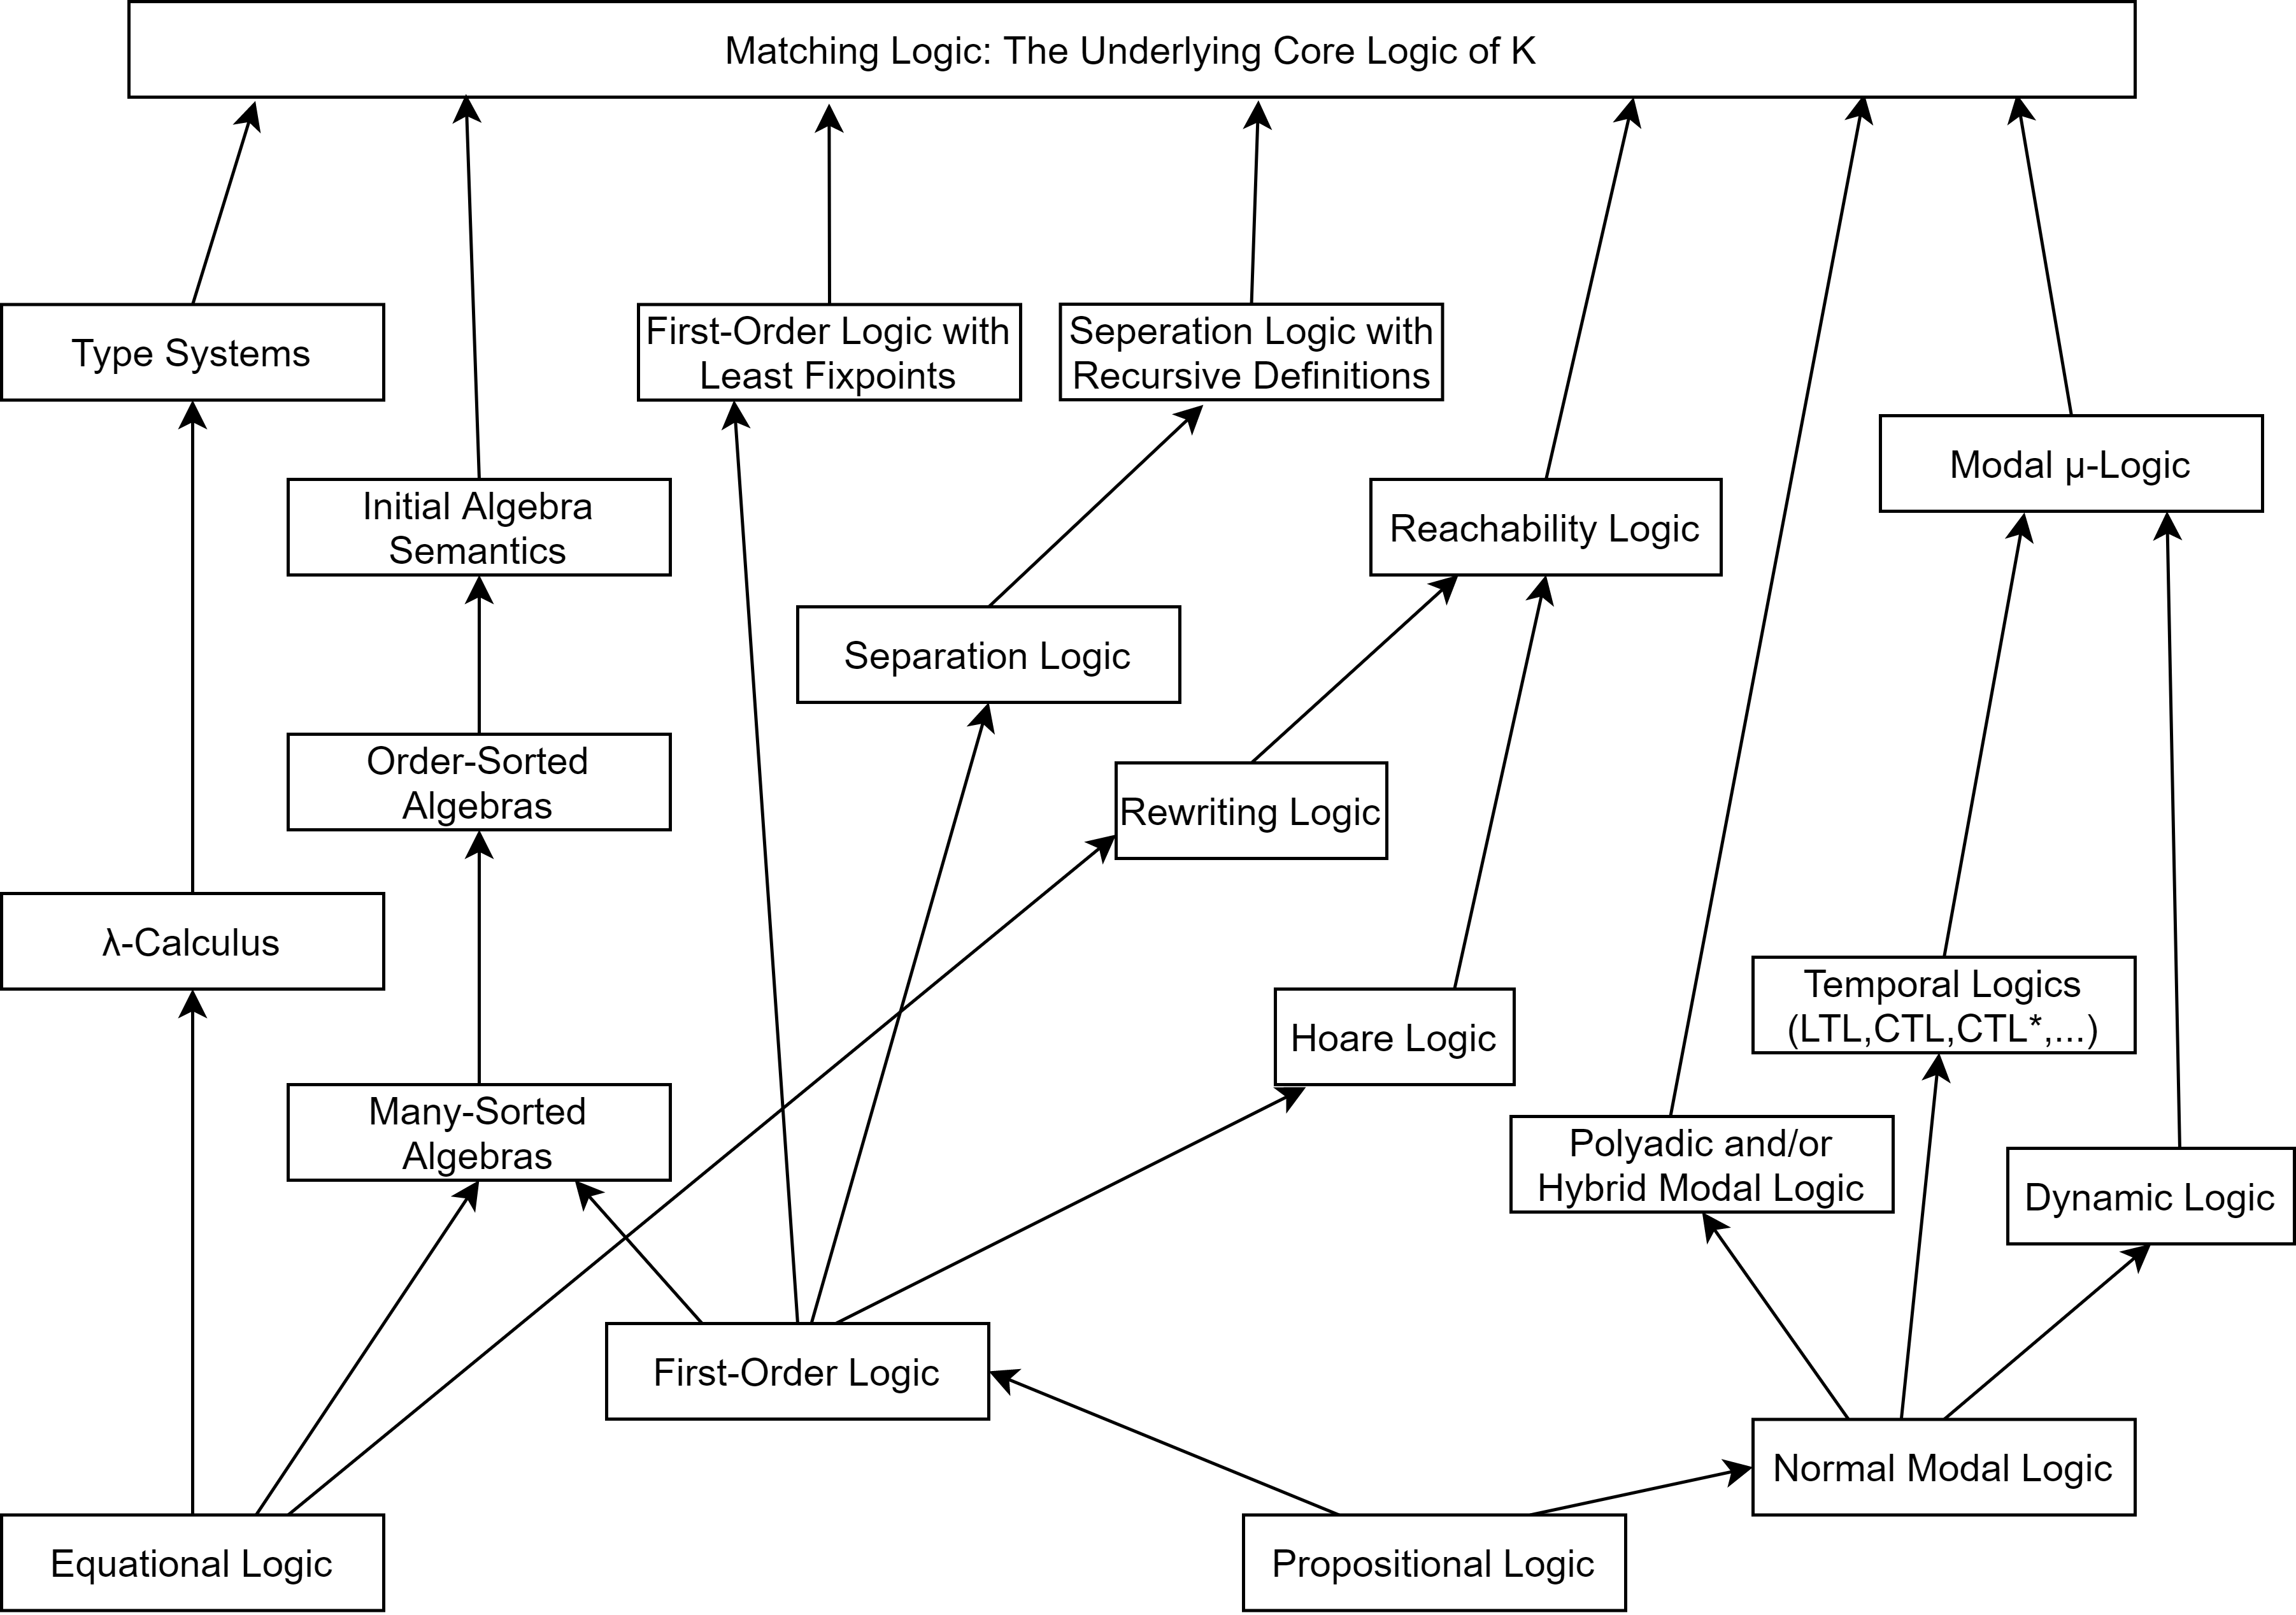
\includegraphics[width=0.9\columnwidth]{figs/logics.png}
\caption{Many logical systems can be captured by matching logic theories (the figure includes both published and future work).}
\label{fig:logics}
\end{figure}

In the following, I discuss four logical systems and/or formalisms and their 
matching logic theories:
FOL with least fixpoints (LFP),
reachability logic, 
type systems, and initial algebra semantics. 
They are representative approaches to designing formal language semantics. 
In the LFP section, I will show how to define recursive relations and/or 
predicates
using the least fixpoint operator $\mu$ of matching logic. 
In the reachability logic section, I will explain how formal verification,
including the classical Hoare-style verification using Hoare triples,
can be expressed using reachability rules, which can then be defined using 
matching logic patterns, allowing matching logic to deal with formal 
verification of all programming languages based on their formal semantics. 
In the type systems section, I will explain how binders such as $\lambda$
in $\lambda$-calculus can be defined using matching logic, where the binding 
behavior of $\lambda$ and any other binders is obtained for free
from the binding behavior of the built-in binder $\exists$ in matching logic.
Finally, in the initial algebra semantics, I will firstly show how sorts, 
many-sorted algebras, and order-sorted algebras can be axiomatically defined in 
matching logic and then discuss the matching logic definition of initial 
algebras. 

\paragraph{FOL with least fixpoints (LFP).}
LFP is a popular system that is used to specify and reason about 
induction, recursion, and fixpoints. 
LFP extends the classical first-order logic by \emph{fixpoints} 
and allows formulas of the form
$
[\lfp_{R,x} \varphi](t)
$,
where $R$ is a \emph{recursive relation symbol}, $x$ is an argument of $R$, 
$\varphi$ is a formula where $R$ and $x$ can (recursively) occur, and $t$ is a 
term. 
Here, $[\lfp_{R,x} \varphi]$ denotes the smallest relation $R$ such that
$\forall x \ld R(x) = \varphi$. 

LFP defines fixpoints differently than matching logic, which only allows the 
definitions of \emph{recursive sets} using the least fixpoint operator $\mu$:
intuitively, the matching logic pattern $\mu X \ld \varphi$ denotes the 
smallest set $X$ such that $X = \varphi$. 
To capture LFP recursive relations, we need to reduce them to recursive sets. 

In \cite{CR19}, I showed that $[\lfp_{R,x} \varphi]$ can be defined in terms of 
its \emph{indicator set} $I_R$, which is the set of arguments $y$ 
such that $[\lfp_{R,x}](y)$ holds.
The indicator set $I_R$ is a recursive set and can be defined by the following 
pattern:
$$
I_R = \mu R \ld \exists x \ld x \land \varphi
$$
where, intuitively, $\exists x \ld x \land \varphi$ denotes the set of all $x$ 
such that $\varphi$ holds. 
Here, we tacitly regard all occurrences of $R(t)$ in $\varphi$ 
as the predicates $t \in R$, which state that $t$ belongs to the indicator set 
$R$.  
This way, I proved that LFP can be defined in matching logic 
and $I_R$ defined above yields the same semantics as $[\lfp_{R,x}]$ in LFP. 

\paragraph{Reachability logic and Hoare logic.}

Reachability logic aims at sound and (relatively) 
complete formal verification of all programming languages based on their 
operational semantics. 
In reachability logic, the formal semantics of a language $L$
is defined by a set of \emph{rewrite rules} $S = \{ \varphi_i \To 
\varphi'_i \mid 1 \le i \le n\}$, where $\varphi_i$ and $\varphi'_i$ are 
patterns matched by program states, called \emph{configurations}. 
One fixed set of \emph{reachability proof rules} is used to  
derive reachability judgments of the form $S \vdash \psi \To \psi'$, meaning 
that any 
configurations that matches $\psi$ will eventually reach $\psi'$,
unless the execution diverges;
this yields \emph{partial correctness}.
As a special instance, a Hoare triple
$\{\varphipre\} \, \mathit{code} \, \{\varphipost\}$ can be expressed by the 
following reachability rule:
$$
\cell[cfg]{\cell[code]{\mathit{code}} \cdots} \land \varphipre
\To \cell[cfg]{\cell[code]{\mathit{skip}} \cdots} \land \varphipost
$$
where the left-hand side consists of the program ``$\mathit{code}$''
and the pre-condition $\varphipre$
and the right-hand side consists of no remaining code
(represented by ``$\mathit{skip}$'') and the post-condition $\varphipost$. 
An important characteristic of reachability logic is that it uses one 
\emph{fixed} set of proof rules to obtain sound and (relative) complete formal 
verification for all programming languages, given that their formal semantics 
are defined by a set of rewrite rules. 
Reachability has been the logical foundation of the current \K's formal 
verification tools.

In \cite{CR19}, I proved that reachability logic can be defined in matching 
logic and all reachability proof rules can be proved as matching logic theorems 
using the proof system in \Cref{fig:ps}. 
In particular, reachability rules are defined as follows:
$$
\varphi_1 \To \varphi_2 \equiv \varphi_1 \imp 
\left(\nu X \ld \varphi_2 \vee \onenext X\right)
$$
where $\nu$ is the greatest fixpoint operator that can be defined from the 
least fixpoint operator $\mu$ and $\onenext$ is a matching logic symbol called 
``one-path next'': $\onenext X$ denotes the set of states that have (at least) 
a next state that matches $X$. 
I showed that the above definition works and yields the same 
partial-correctness semantics of reachability rules. 
This way, I proved that matching logic can replace reachability logic 
as the more uniform logical foundation of \K and its formal verification tools. 



\paragraph{Type systems.}

$\lambda$-calculus \cite{Chu41} and type systems are one of the foundations of 
computation.
In $\lambda$-calculus, computations are defined in terms of \emph{function 
abstraction} $\lambda x \ld e$, where $\lambda$ is a binder that binds $x$ in 
the function body $e$. 
Function application is defined by the following famous \BETA rule:
$$
\BETA \quad (\lambda x \ld e) e' = e[e'/x]
$$

In \cite{CR20}, I proved that $\lambda$-calculus and many type systems
can be defined in matching logic. 
The main difficulty lies in the treatment of \emph{binders}. 
Indeed, if we simply define $\lambda$ as a binary function, then the binding 
behavior of $\lambda$ such as $\alpha$-equivalence and capture-avoiding 
substitution needs to be defined separately. 
If there are multiple binders, each of them 
needs to have its own $\alpha$-equivalence 
and capture-avoiding substitution defined separately, leading to duplication. 
I proposed a novel definition of binders where the binding behavior 
is obtained for free by the built-in binder $\exists$ in matching logic:
$$
\lambda x \ld e \equiv \lam \ \underbrace{(\intension \ (\exists x \ld 
\pr{x,e}))}_{\text{graph of function $x \mapsto e$}}
$$
Intuitively, $\intension \ (\exists x \ld \pr{x,e}))$ returns the graph
of the function that maps $x$ to $e$. 
Note that $x$ is bound by the $\exists$ binder in the above, so the binding 
behavior of $\lambda$ is inherited from the binding behavior of $\exists$. 
Then, I applied the same idea to other logical systems with binders,
including type systems such as the pure type systems \cite{MP93,vBJut93,Bar93} 
and System~F \cite{Gir86,CMMS94} as well as other systems with binders such as 
$\pi$-calculus \cite{MPW92}. 

\paragraph{Initial algebra semantics.}



Initial algebra semantics \cite{GTWW77} is a main approach to formal 
language semantics based on algebraic specifications and their 
initial models.
It has led to extensive research on its theories and applications
\cite{GWM+00,CDE+20,DF98,agda-ias,ASF+SDF,CASL}.
The key idea is to define the sorts of data and the operations on the data
as an algebraic specification $E$.
Among all algebras that satisfy $E$, 
there is an \emph{initial algebra} $I$, unique up to isomorphism,
such that for any other algebra $A$ satisfying $E$
there is a unique morphism $h_A \colon I \to A$. 
In this view, the syntax of a programming language {forms} 
an initial algebra and its formal semantics is a way to associate the syntax 
with the 
\emph{intended} semantic model (algebra).
The unique morphism $h_A$ \emph{is} the semantic function mapping syntax to 
semantics. 
%As an example, the Scott-Strachey denotational semantics~\cite{Sco82}
%uses complete partial orders as the intended semantic models, and
%inductively defines denotations for each syntactic constructs
%to be the unique morphisms.
Initiality has a close relationship with \emph{induction}.
Since program syntax is often defined inductively, the initial algebra $I$
enjoys the \emph{principle of induction}, which can then be mapped to the 
semantic models through the unique morphisms. 
%Note that this use of the initiality often occurs without being 
%noticed; e.g. when we apply ``structural induction on program syntax'' to 
%prove 
%``properties about the semantic models'',
%we are mapping the inductive reasoning on the initial algebra (program syntax) 
%to its semantics,  via the unique morphism.

In \cite{CLR20}, I proved that initial algebra semantics can be defined in 
matching logic. 
Firstly, I showed that many-sorted and order-sorted algebras can be defined in 
matching logic in an axiomatic way. 
Formally speaking, a many-sorted algebra $A$
consists of a set of sorts $s_1$, $s_2$, \dots 
whose corresponding carrier sets in $A$ are written
$A_{s_1}$, $A_{s_2}$, \dots, respectively.
In addition, $A$ includes a set of sorted functions
$f \colon s_1 \times \dots s_n \to s$ whose interpretations
are functions $f_A \colon A_{s_1} \times \dots \times A_{s_n} \to A_s$. 
Matching logic is an unsorted logic and has no built-in support for sorts, but 
it can define sorts and the sorts related concepts in an axiomatically way. 
For each sort $s$, we define a matching logic symbol also written $s$ to 
represent its sort name. 
Then, we introduce an \emph{inhabitant symbol} $\inh{\_}$ to get the carrier 
set of a sort $s$ by applying it to $s$
as in $\inh{\_}\,s$, or written $\inh{s}$. 
The nonempty-ness of the carrier sets and the signatures of many-sorted 
functions can be axiomatized by patterns as follows:
\begin{align*}
& \inh{s} \neq \bot & \text{\Slash the carrier set of $s$ is nonempty} \\
& \forall x_1 \cln s_1 \dots \forall x_n \cln s_n \ld \exists y \cln s \ld
f \, x_1 \, \dots \, x_n = y
& \text{\Slash $f$ is a many-sorted function}
\end{align*}
where the \emph{sorted quantification} can also be defined by patterns:
$$
\forall x \cln s \ld \varphi \equiv \forall x \ld x \in \inh{s} \imp \varphi
\qquad\qquad \exists x \cln s \ld \varphi \equiv \exists x \ld x \in \inh{s} 
\land \varphi
$$
Order-sorted algebras can be defined in a similar, axiomatic way. 
In particular, the subsorting relation $s_1 < s_2$ is axiomatized by
the following pattern:
$$
\inh{s_1} \subseteq \inh{s_2} \qquad\qquad \text{\Slash $s_1$ is a subsort of 
$s_2$}
$$

Initiality is defined using the least fixpoint operator $\mu$. 
For example, the initial algebra that has one sort $\Nat$
and two constructors $\zero$ and $\suc$ can be defined by the following patterns
following the famous ``no-junk no-confusion'' slogan:
\begin{align*}
& \inh{\Nat} = \mu N \ld \zero \vee \suc(N) & \text{\Slash no-junk}\\
& \forall x \cln \Nat \ld \zero \neq \suc(x) & \text{\Slash no-confusion, 
different constructors}\\
& \forall x \cln \Nat \ld \forall y \cln \Nat \ld 
\suc(x) = \suc(y) \imp x = y
& \text{\Slash no-confusion, same constructor}
\end{align*}
This way, I internalized initial algebra semantics in matching logic.


\subsection{Automated Fixpoint Reasoning for Matching Logic}
\label{sec:mlprover}

Given the expressiveness of matching logic, it is highly desirable that we 
develop an \emph{automated theorem prover} for matching logic, as it can be 
instantiated by the various logical theories that we defined in 
\Cref{sec:ml-expressiveness} and obtained specialized provers for  
many logical systems.

In \cite{CTR20}, I developed a prototype matching logic prover,
with a focus on the reasoning about fixpoints and contexts. 
\Cref{fig:pf} illustrates the prover architecture.
It is based on matching logic, upon which a set of generic reasoning modules
are implemented for fixpoint reasoning, frame reasoning, context reasoning,
FOL reasoning, and domain reasoning using SMT solvers.
Automated reasoning is implemented as a \emph{proof search} over 
the proof rules of these reasoning modules. 

\begin{figure}
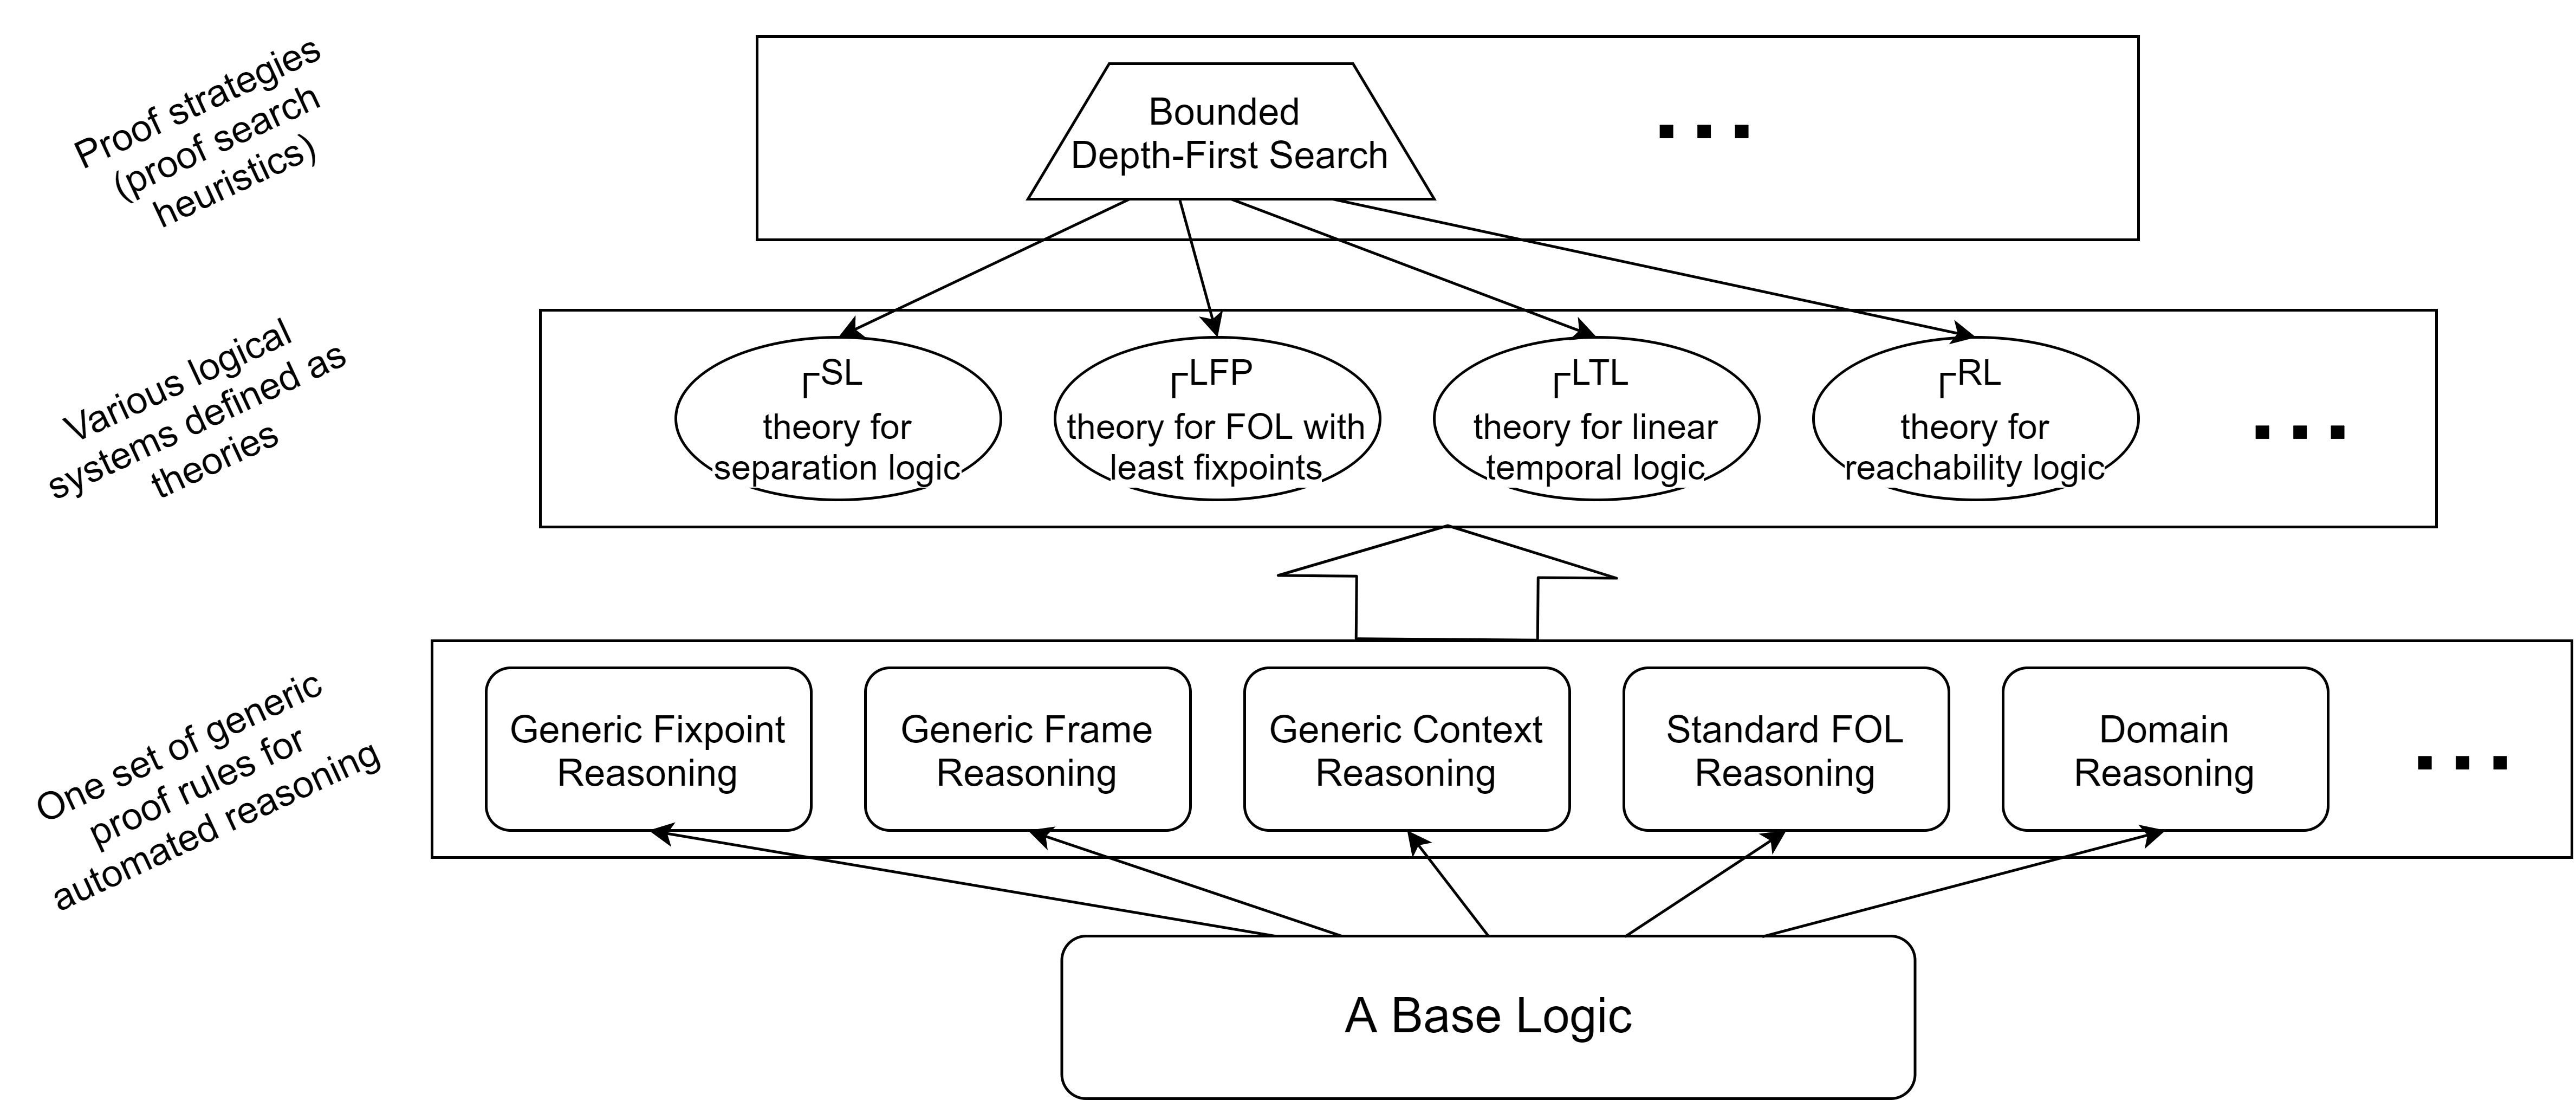
\includegraphics[width=0.9\textwidth]{figs/proofframework.png}
\caption{A unified automated proof framework based on matching 
logic.}
\label{fig:pf}
\end{figure}

The prover can be instantiated by a matching logic theory, resulting in a 
specialized prover for that theory. 
For example, we can instantiate the prover by a theory
$\Gamma^\SL$ that defines separation logic \cite{Rey02} and the result is a 
separation logic prover. 
In \cite{CTR20}, I carried out an experiment and instantiated the prover
by four matching logic theories
that define LFP, separation logic, linear temporal logic (LTL), and 
reachability logic, respectively. 
The experiment results were promising, showing that the specialized provers
have competitive effectiveness compared to the state of the art.
For example, the separation logic prover instantiated by $\Gamma^\SL$
was able to resolved 265 out of 280 obligations in the official SL-COMP 2019 
benchmark, which would have ranked it the third place if it participated in the 
competition. 


%In this paper we present a prototype implementation of a unified proof 
%framework
%for automating fixpoint reasoning.
%As base logic we choose \emph{matching logic}, which was recently proposed
%as a foundation for a variety of logical systems, including FOL with least
%fixed-points, modal and temporal logics, separation logics,
%etc.~\cite{Ros17,CR19}.
%Besides expressiveness, an advantage that matching logic offers is its compact
%syntax and convenient notation through its {\em patterns}
%(Section~\ref{sec:prelim}), which allow us to encode formulae in other logical
%systems almost verbatim.
%For example, the matching logic encoding of modal logic defines a symbol
%$\eventually\_$
%which allows us to encode modal logic formula $\eventually p$ as matching logic
%pattern
%$\eventually p$, with essentially zero representational distance; this is in
%sharp
%contrast to how modal logic is encoded in FOL~\cite{BRV01}, e.g., where a 
%binary
%predicate needs to be added and quantifiers in the resulting FOL formula.



%To evaluate our unified proof framework and prototype implementation, we
%consider four representative logical systems for fixpoint reasoning:
%(1) first-order logic extended with least fixpoints~\cite{GS85}, abbreviated
%LFP;
%(2) separation logic extended with recursive definitions~\cite{Rey02,CDNQ12},
%abbreviated SL;
%(3) linear temporal logic~\cite{Pnu77}, abbreviated LTL; and
%(4) reachability logic~\cite{RSCM13}, abbreviated RL.
%LFP is the canonical logic for fixpoint reasoning in the first-order domain.
%SL is the representative logic for reasoning about data-manipulating programs
%with pointers;
%LTL is the temporal logic of choice for model checkers of
%infinite-trace systems, e.g., SPIN~\cite{Hol97}.
%RL is a language-parametric generalization of Hoare
%logic~\cite[Section~4]{SPY+16},
%where the programming language semantics is given as an input theory and
%partial correctness is
%specified and proved as a reachability rule $\varphi_\textit{pre} \To
%\psi_\textit{post}$.
%These four logics therefore represent relevant instances of fixpoint reasoning
%across
%different and important domains.
%We believe that they form a good benchmark for evaluating a unified proof
%framework for fixpoint reasoning, so we set ourselves the long-term goal to
%support
%{\em all} of them.
%We will give special emphases to separation logic (SL) in this paper, however,
%because it
%gathered much attention in recent years that resulted in several automated SL
%provers
%and its own international competition SL-COMP'19~\cite{SNPR+19}.

%It would be unreasonable to hope at such an incipient stage that a generic
%automated prover can be superior to the state-of-the-art domain-specific 
%provers
%and algorithmic decision procedures for all four logics, on all existing
%challenging benachmarks in their respective domains.
%Therefore, for each of the domains, we set ourselves a limited objective.
%For SL, the goal was to prove all the 280 benchmark properties collected by
%SL-COMP'19
%in the problem set \texttt{qf\_shid\_entl} dedicated to inductive reasoning.
%For LTL, the goal was to prove the axioms about the modal operators
%``always'' $\always \varphi$ and ``until'' $\varphi_1 \until \varphi_2$
%(whose semantics are defined as fixpoints) in its complete proof system.
%For LFP and RL, our goal was to verify a simple imperative program \texttt{sum}
%that computes the total of $1$ to input $n$ using both the LFP and RL
%encodings,
%and show that it returns the correct sum $n(n+1)/2$ on termination.
%We report what we have done in pushing towards the above goals, and
%discuss the difficulties that we met, and the lessons we learned.

%\subsubsection{An Overview of Our Unified Proof Framework}
%\label{sec:overview_framework}
%
%Our unified proof framework consists of three main reasoning modules:
%fixpoint, frame, and context (also illustrated in Fig.~\ref{fig:pf}).
%The fixpoint reasoning module is the main one; the other two are to help
%fixpoint reasoning work properly.
%Note that these three modules are generic, that is, they work with all
%matching logic theories.
%Therefore, they accomplish fixpoint reasoning, frame reasoning, and context
%reasoning for {\em all} logical systems defined as theories in matching logic.
%
%The main challenge we faced while developing our unified proof framework was
%that
%the existing proof system of matching logic~\cite{CR19} is too fine-grained to
%be amenable for automation.
%For example, its \prule{Modus Ponens} proof rule
%``$\vdash \varphi \imp \psi$ and $\vdash \varphi$ implies $\vdash \psi$''
%requires the prover to guess a premise $\varphi$, which does not bode well with
%automation.
%%Its support for first-order reasoning is two (modified) proof rules borrowed
%%from
%%FOL proof system and is highly cumbersome to use.
%%For example, the common substitution rule
%%$\vdash (\forall x \ld \varphi) \imp \varphi[t/x]$ for term $t$ requires a
%%proof propositional to the
%%size of $t$; see~\cite[Lemma~61]{CR19a}.
%Most importantly, its \prule{Knaster-Tarski} proof rule
%(also called Park induction~\cite{E97}) for fixpoint reasoning
%\begin{center}
%		$\prule{Knaster-Tarski} \quad \begin{array}{c}\begin{prftree}
%		{ \varphi[\psi/X] \imp \psi }
%		{(\mu X \ld\varphi) \imp \psi}
%		\end{prftree}
%		\end{array}$
%\end{center}
%is limited to handling the cases where the LHS of the proof goal
%is a standalone least fixpoint.
%It cannot be directly applied to proof goals in LFP or SL,
%such as $\lsegleft(x,y) \sand \lst(y) \imp \lst(x)$ (see Section~\ref{sec:ic}),
%where the LHS $C[\lsegleft(x,y)]$ contains the fixpoint $\lsegleft(x,y)$
%within a context $C[\hole] \equiv \hole \sand \lst(y)$.
%An indirect application is possible \emph{in theory}, but it involves
%sophisticated, ad-hoc reasoning to eliminate the context $C$ from the LHS,
%which cannot be efficiently automated.
%
%Our fixpoint module addresses the above challenge by
%proposing a context-driven fixpoint proof rule, \prule{kt}, shown in
%Fig.~\ref{fig:lfprule}, which is a sequential composition of
%several proof rules that first \prule{wrap} context $C$ within the RHS $\psi$,
%written $\ic{C}{\psi}$, and eliminate
%it from the LHS, then apply inductive reasoning, and finally 
%\prule{unwrap} context $C$ and restore it on the LHS.
%The pattern \(\ic{C}{\psi}\), called {\em contextual implication}, is 
%expressible
%in matching logic and intuitively defines all the elements which in context
%$C$ satisfy $\psi$.
%%In other words, \prule{kt} and the new fixpoint module systematically support
%%generic fixpoint reasoning within any context.
%%
%%The other two reasoning modules, frame reasoning and context reasoning, are
%%important
%%supplements to the fixpoint reasoning module.
%The fixpoint module therefore makes contexts explicitly occur as conditions
%in proof goals.
%Sometimes the context conditions are needed to discharge a proof goal,
%other times not.
%The frame and context reasoning modules help to eliminate contexts from proof
%goals.
%Specifically, frame reasoning is used when the context is unnecessary:
%it reduces proof goal $\vdash C[\varphi] \imp C[\psi]$ to $\vdash \varphi \imp
%\psi$.
%On the other hand, context reasoning is used when the context is needed
%in order to discharge the proof goal, by allowing us to derive
%$\vdash C[\ic{C}{\psi}] \imp \psi$.
%We shall discuss and analyze the frame and context reasoning in detail in
%Section~\ref{sec:algo}.
%
%We have not implemented any smart proof strategies or proof search heuristics,
%but only a naive bounded depth-first search (DFS) algorithm.
%Our evaluation on the SL-COMP'19 benchmark shows that the naive bounded-DFS
%strategy
%can prove 90\% of the properties without frame reasoning, and 95\% with frame
%reasoning
%(Section~\ref{sec:eval}).
%This was surprising, because it would place our generic proof framework
%in the third place in the SL-COMP'19 competition, among dozens of specialized
%provers
%developed specifically for SL and heap reasoning.
%However, the remaining 5\% properties appear to require complex, SL-specific
%reasoning,
%which is clearly beyond the ability of our generic framework.
%We have also considered only a small number of LFP and LTL proofs, which could
%all be
%done using the same simplistic bounded-DFS strategy; more powerful proof
%strategies
%will certainly be needed for more complex proofs and will be developed as part
%of
%future work.

\subsection{Known Results about Matching Logic Complete Deduction}
\label{sec:known-complete}

A completeness theorem establishes the connection between the semantic validity 
relation $\Gamma \vDash \varphi$ and the provability relation $\Gamma \vdash 
\varphi$. 
Intuitively, $\Gamma \vDash \varphi$ states that all matching logic models
that satisfy the axioms in $\Gamma$ also satisfy $\varphi$,
while $\Gamma \vdash \varphi$ states that there exists a formal proof
using the proof system in \Cref{fig:ps} 
to prove $\varphi$ from the axioms in $\Gamma$. 
The connection  between them can be illustrated as the following 
soundness/completeness 
properties:
$$
\Gamma \vDash \varphi \xleftrightarrows[\text{completeness}]{\text{soundness}}
\Gamma \vdash \varphi
$$
Soundness has been proved in \cite{CR19} but completeness is more involved. 

In general, matching logic does not have complete deduction. 
This means that for any (effective) proof system, the above completeness 
property will fail for some $\Gamma$ and $\varphi$. 
The reason for that is that matching logic supports FOL-style quantification 
as well as the least fixpoints. 
We can thus define a theory $\Gamma^\Nat$ that captures precisely the 
standard model of natural numbers with addition and multiplication. 
By Godel's first incompleteness theorem \cite{Goe92}, 
there does not exists an effective proof system that is complete for
the theory $\Gamma^\Nat$. 
However, it is still possible that the proof system in \Cref{fig:ps} is 
complete for a fragment of matching logic.

In \Cref{tab:summary}, I summarize the known results and open problems about matching logic complete deduction (as well as its decidable fragments and small model properties, which will be discussed as proposed work in \Cref{sec:proposed}).
Since matching logic does not have complete deduction in general, I studied its
\emph{syntactic fragments} that include only a subset of the syntactic constructs
of matching logic. 
In \Cref{tab:summary}, I use $\{\}$ to denote the fragment of matching logic that includes only symbols, application, and the propositional connectives
$\bot$ and $\imp$. 
I use $\cex$ to mean element variables and the $\exists$ quantification
and use $\cmu$ to mean set variables and the $\mu$ least fixpoint operator.
Therefore, $\{\cex,\cmu\}$ denotes the full matching logic with all the syntactic constructs.

\newcommand{\tagaa}{1} 
\newcommand{\tagab}{2} 
\newcommand{\tagac}{3} 
\newcommand{\tagad}{4} 
\newcommand{\tagcc}{1} 

\begin{table}
\caption{A summary of the known results (denoted \cmark and \xmark) and open problems
(denoted \qmark) about matching logic, including its complete deduction, decidable fragments, and small model properties.}
\label{tab:summary}
\centering
\vspace{\baselineskip}
\begin{tabular}{lccccc}
\textbf{Properties} &
\multicolumn{4}{c}{\textbf{Syntactic Fragments of Matching Logic}} \\
& $\{\}$
& $\{\cmu\}$
& $\{\cex\}$
& $\{\cmu,\cex\}$
\\\hline
Completeness (for the empty theory) & \cmark & \qmark & \cmark & \qmark \\
Completeness (for all theories)  & \qmark & \qmark & \cmarkx$^\tagcc$ & \xmark 
\\
\hline
Decidability (for the empty theory)  & \framebox{\cmark} & \framebox{\cmark} & \qmark & \qmark 
\\
Decidability (for all theories) & \qmark & \qmark & \xmark & \xmark \\
\hline
Small model property (for the empty theory)  & \cmark & \framebox{\cmark} & \qmark & \qmark \\
Small model property (for all theories) & \xmark & \xmark & \xmark & \xmark \\
\hline
\end{tabular}
\begin{flushleft}\footnotesize
The framed check marks \framebox{\cmark} indicate results that have been proved but not yet published, which will be discussed as proposed work in \Cref{sec:proposed}.\\$\hat{}$\,\tagcc. Only proved for theories that define equality, inspired by \cite{Ros17}.
\end{flushleft}
\vspace{1ex}
\label{tab:op}
\end{table}

I call the fragment denoted by $\{\cex\}$ the \emph{fixpoint-free fragment},
because it excludes set variables and fixpoints. 
In \cite{CR19}, I proved two completeness results for the fixpoint-free 
fragment of matching logic. 
The first completeness result shows that all valid patterns can be 
proved from the proof system in \Cref{fig:ps}. 

\begin{theorem}
\label{thm:completeness-local}
Consider the fixpoint-free fragment of matching logic. 
The proof system in \Cref{fig:ps} is complete for the empty theory, that is,
$\emptyset \vDash \varphi$ implies $\emptyset \vdash \varphi$. 
\end{theorem}

Then, I pushed the above theorem further to theories where \emph{equality} is 
(axiomatically) defined. 

\begin{theorem}
\label{thm:completeness-defined}
Under the condition in \Cref{thm:completeness-local}, the proof system is 
complete for any theory $\Gamma$ that defines equality.
%that is, $\Gamma \vDash \varphi$ implies $\Gamma \vdash \varphi$.
\end{theorem}

These completeness results are not of theoretical interest only. 
They are evidence that show that the proof system in 
\Cref{fig:ps} is not ad-hoc. Instead, it is closely related to the semantics 
and the validity relation. 

Future work on the completeness of matching logic based on Henkin semantics 
is explained in 
\Cref{sec:proposed-complete}. 
Future work on the decidable fragments of matching logic as well as the small model properties is explained in \Cref{sec:proposed-decision}.


\section{Proposed Work}
\label{sec:proposed}

In this section, I discuss technical details of the proposed research. 

%\subsection{Matching Logic Interactive Prover}
%\label{sec:proposed-mlip}
%
%Matching logic interactive prover (MLIP) allows users to define matching logic 
%theories using an intuitive and user-friendly frontend language
%and to prove formal theorems within the theories using a high-level strategy 
%language. 
%MLIP forms an important piece in the proposed formal language framework
%as it provides the ultimate reasoning power to carry out formal proofs in 
%matching logic. 
%
%\paragraph{MLIP frontend.}
%
%MLIP frontend language allows users to define
%a matching logic theory (consisting of a set of symbols and a set of axioms)
%and to declare theorems and their formal proofs. 
%
%MLIP consists of four main components:
%a frontend, a proof strategy language, a backend, and 
%
%\paragraph{MLIP Frontend}
%
%\paragraph{MLIP Proof Strategies}

\subsection{Matching Logic Proof Checker}
\label{sec:proposed-mlpc}

As shown in \Cref{fig:ps}, the matching logic proof system is a Hilbert-style 
proof system that derives judgments of the form
$\Gamma \vdash \varphi$. 
Formally, a Hilbert-style proof within a theory $\Gamma$ has the form
$\pr{\Gamma : \varphi_1 \varphi_2 \cdots \varphi_k}$ such that
for each $1 \le i \le k$, 
$\varphi_i$ is an axiom (in the proof system or in $\Gamma$)
or it is the result of applying a proof rule on the patterns that appear before 
$\varphi_i$. 
We can annotate how each $\varphi_i$ is proved along with the Hilbert-style 
proof and the resulting annotated proof,
written $\pr{\Gamma : \varphi_1,\dots,\varphi_k}_\obj$, is called a \emph{proof 
object}.
A \emph{proof checker} is an algorithm that takes a proof object as input and 
checks whether it encodes a correct Hilbert-style proof. 
The following are the key properties that a proof checker and the proof objects 
should satisfy:
\begin{description}
\item[Correctness.]
If $\PC\left( \pr{\Gamma : \varphi_1,\dots,\varphi_k}_\obj \right) = 
\text{true}$ then $\Gamma \vdash \varphi_k$.
\item[Effectiveness.]
If $\Gamma \vdash \varphi_k$ then
there exist a proof object $\pr{\Gamma : \varphi_1,\dots,\varphi_k}_\obj$
such that $$\PC\left( \pr{\Gamma : \varphi_1,\dots,\varphi_k}_\obj \right) = 
\text{true}$$
\end{description}

In the following, I briefly discuss how to create proof objects
$\pr{\Gamma : \varphi_1,\dots,\varphi_k}_\obj$ and implement
the proof checker using a formal language called Metamath \cite{metamath}. 

\subsubsection{Metamath Overview}
\label{sec:metamath}
 
Metamath is a simple formal language that can define the meta-theory of a 
logical system and prove meta-theorems about it, accompanied by proofs that can 
be verified by a computer program, called a {Metamath proof verifier}. 
At its core, Metamath is a substitution system. 
The main data that Metamath manipulates is that of a sequence of Metamath tokens, which are either Metamath constants or Metamath variables.\footnote{Although verbose, we keep the premodifier ``Metamath'' so as not to confuse with the concepts in matching logic.} 
A Metamath variable can be substituted for a sequence of Metamath tokens that may include both Metamath variables or Metamath constants. 
Metamath allows users to define certain Metamath token sequences as Metamath axioms,
from which, by substitution, more Metamath token sequences can be obtained, i.e. ``proved'', as Metamath theorems. 
A Metamath proof of a Metamath theorem is essentially an encoding of the substitution operations that have been applied in order to obtain the proved theorem. 
Although Metamath also has a few other features,
such as supporting sorts and 
allowing to declare two Metamath variables as ``distinct'' (whose formal meaning is not important here),
what was described above covers the core functionality of Metamath. 

A Metamath proof verifier takes a Metamath theorem and its proof and applies the substitution operations specified in then proof to see if the result is the same as the theorem. 
The main advantage of Metamath, which is also the main reason I decide to implement the first prototype of the matching logic proof checker in it, 
is its simplicity and efficiency. 
This is explained later. 
Before that, I explain how Metamath is used to define a logic $L$
and to prove the meta-theorems of $L$.

The way how Metamath is used to define a logic $L$ and to prove the meta-theorems of $L$ is explained below. 
A Metamath definition that consists of the following basic components is prepared:
\begin{enumerate}
\item A Metamath definition of $L$:
\begin{enumerate}
\item a declaration of some Metamath constants that are used to represent the 
logical constructs of $L$, the syntactic categories in the syntax of $L$
(such as that of the formulas of $L$) as the sorts in Metamath,
and some meta-level syntax that is needed to state the meta-theorems. A common one is the proof entailment symbol ``$\vdash$'';
\item a declaration of some Metamath variables that are used to represent the meta-variables of $L$;
\item a set of Metamath axioms that define the syntax and proof system of $L$;
\end{enumerate}
\item a set of Metamath theorems, accompanied by their Metamath proofs, which prove the given meta-theorems of $L$.
\end{enumerate}
Intuitively, item 1 forms a specification of a proof checker of $L$ and item 2 forms
a proof object of the given meta-theorems. 
The proof checking function $\PC$ of $L$ is the Metamath proof checking algorithm

Metamath has been successfully applied to formalize many important mathematical logics and/or theories. 
The most substantial work that has been done using Metamath
is a 40-million-LOC formalization of the ZFC set theory axioms
as well as the basic and more advanced mathematics that is defined based on set 
theory, accompanied by 23,000 completely worked out Metamath proofs. 

Metamath is known for its simplicity and efficiency.
Since I am pursuing a similar goal with the matching logic proof checker, I decide to implement the first prototype in Metamath so as to take advantage of the state of the art tools. 
There are more than 15 Metamath proof verifiers, all compact and short. 
In terms of the size, 
the smallest verifier is written in 74 lines of Mathematica code.
Besides that, a Python verifier has 350 lines of code,
a Lua one has 380 lines of code, and a Haskell one has 400 lines of code.
One of the fastest Metamath verifier is written in \Cpp, which can complete the verification of the aforementioned Metamath definition of set theory with 23,000 Metamath proofs in fewer than 20 seconds. 

Next, I describe the Metamath definition of matching logic.



\subsubsection{Matching Logic Proof Checker Implemented in Metamath}
\label{sec:proposed-mm}

I briefly discuss the design of a 245-LOC prototype matching logic proof checker
\cite{ml-checker} written in Metamath. 

Firstly, I define the primitive syntax of matching logic as Metamath 
constants. \\
\verb|    | \verb|$c \bot \imp \app \ex \mu ( ) $.| \\
Here, the Metamath notation ``\verb|$c ... $.|'' is used to declare a list of 
space-separated constants. 
I declare the bottom \verb|\bot|, 
implication \verb|\imp|,
application \verb|\app|,
the existential quantification \verb|\ex|,
and the least fixpoint operator \verb|\mu|. 
I also define the parentheses, \verb|(| and \verb|)|,
to group the syntax. 

Secondly, I define the following syntactic categories of matching logic using 
Metamath constants. \\
\verb|    |
\verb|$c #Pattern #ElementVariable #SetVariable #Symbol #Variable $.| \\
For each syntactic category in the above, I define the meta-variables that range over it.
For example, I define \verb|ps| and \verb|ph| as the meta-variables for 
matching logic patterns as follows: \\
\verb|    |
\verb|vph  $f #Pattern ph $.| \\
\verb|    |
\verb|vps  $f #Pattern ps $.| \\
Here, the Metamath notation ``\verb|$f ... $.|'' is used to declare a 
meta-variable of a given syntactic category. 
The identifiers \verb|vph| and \verb|vps| are given to the meta-variable 
declarations so that the other proofs can refer to them. 

Thirdly, I define some auxiliary predicates on the syntax of matching logic,
such as checking the free occurrences of a variable in a pattern,
which are are necessary because they appear in the side conditions of matching logic proof rules. 
Some of them are also used in defining the pattern syntax, as shown below. 

Fourthly, I define matching logic syntax. 
In Metamath, this means to define which sequences of the Metamath constants 
and/or variables are regarded as members of the syntactic category 
\verb|#Pattern|. 
The following is the Metamath definition of matching logic syntax.\\
\verb|    |\verb|wv $a #Pattern xX $. | \\
\verb|    |\verb|wb $a #Pattern \bot $.| \\
\verb|    |\verb|wi $a #Pattern ( \imp ph ps ) $.| \\
\verb|    |\verb|wa $a #Pattern ( \app ph ps ) $.| \\
\verb|    |\verb|we $a #Pattern ( \ex x ph ) $.| \\
\verb|    |\verb|${ wm.1 $e #NoNegativeOccurrence X ph $.| \\
\verb|    |\verb|   wm   $a #Pattern ( \mu X ph ) $.| \\
\verb|    |\verb|$}| \\
Here, \verb|xX| is a declared meta-variable that ranges over both the element 
and the set variables.\footnote{For simplicity, I do not show the declaration here. 
}
Similarly, \verb|x| and \verb|X| are declared as meta-variables that range over 
the element variables and set variables, respectively. 
In the above definition, I adopt an S-expression style syntax to encode 
matching logic patterns in Metamath. 
Note that in the definition of the syntax of $\mu X \ld \varphi$, it is 
required that $X$ has no positive occurrences in $\varphi$. 

Fifthly, I define matching logic proof system. 
It includes the following definition of the entailment symbol:\\
\verb|    |\verb#$c |- $.# \\
and Metamath axioms that define the matching logic proof rules. 
For example, the following is the Metamath definition of the 
\prule{Modus Ponens} proof rule: \\
\verb|    |\verb#${  pr-mp.1   $e |- ps $.# \\
\verb|    |\verb#    pr-mp.2   $e |- ( \imp ps ph ) $.# \\
\verb|    |\verb#    pr-mp     $a |- ph $.# \\
\verb|    |\verb#$}# 

Finally, I define an equality relation at the meta-level of matching logic so 
that syntactic sugar can be defined and their properties can be formally proved
from the definitions (instead of axiomatized). 

The resulting Metamath definition is a file \mlmm with 245 lines of Metamath 
code that fully implements the meta-theory of matching logic. 
Using this Metamath definition, 
I can write proof objects as Metamath theorems accompanied with their Metamath
proofs. 
For example, the following Metamath theorem states
that the pattern $\varphi \imp \varphi$ is provable for any pattern $\varphi$:\\
\verb|    |\verb#iid $p |- ( \imp ph ph ) $=# \\
\verb|    |\verb#  vph vph wi vph vph vph wi wi vph vph pr-1 # \\
\verb|    |\verb#  vph vph vph wi wi vph vph wi wi vph vph # \\
\verb|    |\verb#  vph wi vph wi wi vph vph vph wi pr-1 vph # \\
\verb|    |\verb#  vph vph wi vph pr-2 pr-mp pr-mp $.# \\
In the above, the Metamath notation ``\verb|$p ... $= ... $.|'' is used to 
state a theorem and its proof. 

%At a high level, a matching logic proof object 
%$\pr{\Gamma : \varphi_1,\dots,\varphi_k}_\obj$ is encoded as a Metamath file
%that consists of the following components in order:
%\begin{enumerate}
%\item The definition of the meta-level of matching logic in \code{ml.mm} as 
%described in \Cref{sec:proposed-mm};
%\item The definition of symbols that occur in $\Gamma$;
%\item The definition of axioms in $\Gamma$;
%\item The proofs of the patterns $\varphi_1,\dots,\varphi_k$.
%\end{enumerate}

\subsubsection{Generating Proof Objects for Program Execution and Verification}

In matching logic, the formal semantics of any programming language $L$ 
is given as a set of reachability rules.
In \Cref{sec:ml-expressiveness}, I show that reachability rules can be defined as matching logic patterns. 
Therefore, the formal semantics of $L$ is given by a set of matching logic axioms. 
Let $\Gamma^L$ denote the resulting matching logic theory that includes the formal semantics of $L$. 

In \Cref{sec:ml-expressiveness} and \cite{CR19},
I also recall that the dynamic properties of programs such as execution and verification can be expressed by patterns. 
For example, that the initial configuration $\varphi_0$ executes to the final configuration $\varphi_{100}$ in 100 steps,
or that the pre-condition $\varphipre$ eventually reaches the post-condition
$\varphipost$ (in a partial-correctness manner), can be expressed by the following matching logic patterns, respectively:
\begin{align*}
& \Gamma^L \vdash \varphi_0 \To^{100} \varphi_{100} &
\Gamma^L \vdash \varphipre \To \varphipost
\end{align*}

To encode the above as proof objects, I need to translate the axioms in $\Gamma^L$ into Metamath axioms that state that each pattern in $\Gamma^L$ is provable. 
The above properties are then stated as Metamath theorems.


\subsection{Matching Logic Complete Deduction}
\label{sec:proposed-complete}

From \Cref{sec:known-complete} we know that 
matching logic has no complete proof system.
If no proof system is complete, how do we know the current proof system
in \Cref{fig:ps} is ``good enough'' and not merely a set of ad-hoc proof rules?
To answer this question, we need to establish a clear and elegant relationship 
between matching logic semantics and matching logic proof system.

\Cref{thm:completeness-local,thm:completeness-defined}  are the completeness results that have been proved for matching logic.
They show that the proof rules in \Cref{fig:ps} 
that handle non-fixpoint reasoning are not ad-hoc
because they are complete with respect to the empty theory and theories where 
equality is present. 
Therefore, the main technical difficulty is the completeness with respect to fixpoints. 


I propose the following method based on \emph{Henkin semantics},
also known as \emph{general semantics}, which gives fixpoint patterns
an alternative semantics. 
In the current semantics, called \emph{standard semantics}, 
the least fixpoint pattern $\mu X \ld \varphi$
is required to be interpreted as the smallest set $X$ such that the equation $X = \varphi$ 
holds (note that $\varphi$ may include $X$).
However, in the proposed Henkin semantics, the least fixpoint
$\mu X \ld \varphi$ is not necessarily interpreted as the true least fixpoint 
in the models. 
Instead, each model $M$ is extended by a nonempty domain
$\DD \subseteq \pset{M}$ as the range of all possible interpretation of the 
fixpoint patterns. 
We call each such pair $\pr{M,\DD}$ a \emph{Henkin model}. 
Least fixpoint pattern $\mu X \ld \varphi$ is then interpreted as the smallest 
set that belongs to $\DD$ such that $X = \varphi$. 
When $\DD = \pset{M}$ is the full power set of $M$, the Henkin model
$\pr{M,\DD}$ yields the standard semantics. 
When $\DD \neq \pset{M}$, Henkin semantics allows to 
have \emph{nonstandard models} where least fixpoints are not interpreted as the 
true least fixpoints in the models but only the least ones in $\DD$. 

The above Henkin extension of the standard semantics is classical and has been 
successfully applied to second-order logic as well as first-order modal 
$\mu$-calculus and has obtained the corresponding completeness results. 




\subsection{Matching Logic Decidable Fragments}
\label{sec:proposed-decision}

Decision procedures play an important role in automated reasoning. 
Matching logic is not decidable, but it has fragments that are decidable.
The simplest fragment is \emph{propositional logic fragment}
that consists of set variables (serving as propositional variables)
and the two propositional connectives $\bot$ and $\varphi_1 \imp \varphi_2$,
and no other constructs. 
However, no further research has been carried out on matching logic 
decidability, which has caused \K to utilize the existing decision procedures 
such as SMT solvers in an ad-hoc way. 

In the proposed research, I will systematically study decidable fragments of 
matching logic and implement the corresponding decision procedures. 
These decision procedures can be integrated into \K and improve the level 
automation in the current \K implementations. 

\paragraph{Satisfiability.}

Firstly, I define the decision problem of matching logic satisfiability modulo 
theory, abbreviated MLSMT, as follows:
\begin{quotation}
Given a theory $\Gamma$ and a pattern $\varphi$, is there a model $M$
and a valuation $\rho$ of variables such that
$M \vDash \Gamma$ and $\ip{\varphi}{M,\rho} \neq \emptyset$, where
$\ip{\varphi}{M,\rho}$ is the interpretation of $\varphi$ in $M$ under $\rho$?
\end{quotation}

MLSMT is an important decision problem. 
It can be used to encode many other interesting and important decision 
problems.
For example, it can be used to encode the following \emph{validity problem}:
\begin{quotation}
Given a theory $\Gamma$ and a pattern $\varphi$, whether $\Gamma \vDash 
\varphi$?
\end{quotation}
Indeed, validity can be solved by calling MLSMT with $\Gamma$ and $\neg 
\varphi$. If $\neg \varphi$ is not satisfiable (modulo $\Gamma$) then
$\varphi$ is valid, and vice versa. 

Another application of MLSMT is to check the \emph{consistency} of a logical 
theory $\Gamma$ in the following sense. 
We call MLSMT with $\Gamma$ and $\top$ 
(called ``top'', defined by $\top \equiv \neg \bot$).
If it returns that $\top$ is satisfiable under $\Gamma$,
we know that $\Gamma$ is not inconsistent because it has a satisfying model. 

\paragraph{Finite/small model property.}

Finite model property is closely related to satisfiability.
It studies the \emph{size} of the satisfying model $M$ of pattern $\varphi$.
Formally, we say that the finite model property holds
if for any $\varphi$ that is satisfiable modulo a theory $\Gamma$,
there exists a satisfying model $M$ whose size is \emph{finite}.
If additionally, the size of $M$ is bounded by $O(f(\abs{\varphi}))$
where $f$ is a computable function and $\abs{\varphi}$ is the size of $\varphi$, we say that the \emph{small model property} holds.
The known results and open problems on small model property 
are summarized in \Cref{tab:summary}.

Finite/small model property is often a byproduct of decidability.
As I show later, decision procedures of MLSMT are based on the tableau method
and build at runtime a satisfying model for the given input pattern $\varphi$ using tableau rules.
The built models have a tree-like structure, possibly infinite, but can be folded into a finite graph-like structure and thus fulfill the finite/small model property.

\paragraph{Syntactic fragments.}

Generally speaking, MLSMT is undecidable for matching logic 
(see \Cref{tab:summary}). 
Therefore, I propose to study 
the \emph{decidable fragments} of matching logic. 
Recall that matching logic has 8 syntactic constructs (\Cref{sec:ml}).
Except $\bot$ and $\varphi_1 \imp \varphi_2$ that build propositional 
constraints as well as user-provided symbols and application, I regard the remaining 4 constructs as optional and denote them using the following tokens:
\begin{enumerate}
\item \(\cev\): element variables;
\item \(\csv\): set variables;
\item \(\cex\): the $\exists$ quantifier; and
\item \(\cmu\): the $\mu$ operator.
\end{enumerate}
A \emph{syntactic fragment} can be described by a subset 
$\Pi \subseteq \{ \cev, \csv, \cex, \cmu \}$ such that
\begin{enumerate}
\item $\cex \in \Pi$ implies $\cev \in \Pi$, and
\item $\cmu \in \Pi$ implies $\csv \in \Pi$. 
\end{enumerate}
Under the above classification,
there are $3 \times 3 = 9$ different syntactic fragments,
where the first $3$ denotes a choice in
$\{ \emptyset, \{\cev\}, \{\cev,\cex\}\}$ and
the second $3$ denotes a choice in
$\{ \emptyset, \{\csv\}, \{\csv,\cmu\}\}$.
In \Cref{tab:summary}, four syntactic fragments are shown. 

\paragraph{Decidability of fragments involving fixpoints.}

It is especially interesting to study decidability when fixpoints are present.
Therefore, I start by studying the
syntactic fragment $\Pi_\mu = \{\csv, \cmu \}$, that is, the fragment of 
matching logic that excludes element variables or the quantification $\exists$,
but allows set variables and least fixpoints. 
Recall that the greatest fixpoints can be defined from least fixpoints and 
negation. 
I also assume that the given theory $\Gamma = \emptyset$. 
Nonempty theories are to be considered in the future, too.

$\Pi_\mu$-fragment can be regarded as an extension of modal $\mu$-calculus, 
whose syntax also 
defines propositional connectives, set variables (called propositional 
variables or atomic propositions) and the least fixpoint operator $\mu$.
The only difference is that modal $\mu$-calculus defines
formulas of the form $\allnext \varphi$ while matching logic defines a binary 
application construct $\varphi_1 \, \varphi_2$. 
This difference can be resolved by defining $\allnext$ as a symbol in matching 
logic and regarding $\allnext \varphi$ as the matching logic symbol/pattern 
$\allnext$ applied to $\varphi$. This way, modal $\mu$-calculus becomes a 
fragment of matching logic $\Pi_\mu$-fragment.


Note that modal $\mu$-calculus is decidable. 
The close relationship between modal $\mu$-calculus and the $\Pi_\mu$-fragment
of matching logic implies that the proof techniques of the decidability of 
modal $\mu$-calculus,
called the \emph{tableau method} \cite{NW96}, 
may be applied to the $\Pi_\mu$-fragment. 
In the tableau method, a set of tableau rules is used to build a satisfying 
model for $\varphi$. 
By construction, the model built by the tableau method has a tree-like 
structure, where each node is associated with a set of patterns that are 
sub-patterns of $\varphi$ and are satisfied by the node. 
This invariant is maintained throughout the construction and is used to prove 
that the resulting model is indeed a satisfying model of $\varphi$. 
In \Cref{fig:tableau}, I list the proposed tableau rules.
I have used the proposed tableau rules to prove following decidability result of matching logic, which is the first decidability result for matching logic of its kind:
\begin{theorem}
MLSMT is decidable for the empty theory $\emptyset$ on the 
$\Pi_\mu$-fragment.
\end{theorem}

\begin{figure}[t]
\begin{align*}
\prule{and}
&\qquad \prftree{\varphi_1 \land \varphi_2 ,
\Gamma}{\varphi_1,\varphi_2,\Gamma}
\\
\prule{or-l}
&\qquad \prftree{\varphi_1 \lor \varphi_2, \Gamma}{\varphi_1,\Gamma}
\\
\prule{or-r}
&\qquad \prftree{\varphi_1 \lor \varphi_2, \Gamma}{\varphi_2,\Gamma}
\\
\prule{ons}
&\qquad \prftree{U, \Gamma}{\varphi[U/X], \Gamma}
\qquad\text{where $U = \kappa X \ld \varphi$ and $\kappa \in
\{\mu,\nu\}$}
\\
\prule{mu}
&\qquad \prftree{\mu X \ld \varphi, \Gamma}{U,\Gamma}
\qquad\text{where $U = \mu X \ld \varphi$}
\\
\prule{nu}
&\qquad \prftree{\nu X \ld \varphi, \Gamma}{U,\Gamma}
\qquad\text{where $U = \nu X \ld \varphi$}
\\
\prule{app-1}
&\qquad \prftree
{\Gamma}{\left\{ \Gamma \fl
\app(\varphi_1,\varphi_2)
 \mid \app(\varphi_1,\varphi_2) \in \Gamma \right\} }
\\
\prule{app-2}
&\qquad \prftree{\Gamma \fl \app(\varphi_1,\varphi_2)}
{ \Gamma \fl \app(\varphi_1,\varphi_2) \fl \left( \Gapa, \Gapb \right) }
\\
\prule{app-3}
&\qquad \prftree{\Gamma \fl \app(\varphi_1,\varphi_2) \fl \left( \Gapa, \Gapb 
\right) } {\left\{ \varphi_i, \Gamma_{\overline{\app},i} \mid i \in \{1,2\} 
\right\}}
\end{align*}
\caption{The proposed tableau rules for the $\Pi_\mu$-fragment that yield decidability.}
\label{fig:tableau}
\end{figure}




\subsection{Defining Logical Systems in Matching Logic}
\label{sec:proposed-logics}

Apart from the logical systems in \Cref{fig:logics}, 
there are still many important logical systems that have not been defined as 
matching logic theories. 

In this proposed work, I plan to consider two logical systems
and define them in matching logic.
They are separation logic and hyper linear temporal logic (hyperLTL).

\paragraph{Separation logic.}

Separation logic \cite{Rey02} was initially proposed to specify and reason about 
data structures on heaps and has developed into a family of logics that deal 
with resources in a computing system.
For example, Iris \cite{iris} is a framework where resources and their 
ownership can be formalized. 

The vanilla separation logic as proposed in the original paper \cite{Rey02}
uses the following syntax to build \emph{heap assertions}:
$$
\varphi \Coloneqq \text{(FOL syntax)}
\mid \emp \mid l \mapsto v \mid \varphi_1 \sand \varphi_2 \mid
\varphi_1 \simp \varphi_2
$$
Semantically, a heap is a finite mapping  $h \colon L \pto V$
where $L$ is a set of locations and $V$ is a set of values. 
There is a distinguished location $\nil \in L$ that denotes the nil location.
Any heap $h$ must be undefined on $\nil$. 
Empty heap $\empheap$ is undefined everywhere. 

Given a valuation $\rho$ of the variables appearing in a heap assertion 
$\varphi$, 
we define the semantic relation
$h,\rho \vDashSL \varphi$ to mean that $h$ satisfies $\varphi$ under $\rho$. 
In the syntax of separation logic, 
$\varphi_1 \sand \varphi_2$ is called separating conjunction and 
$\varphi_1 \simp \varphi_2$ is called separating implication. 
These are the two most important constructs in separation logic. 
The semantics of separating conjunction states that any heap $h$
such that $h,\rho \vDashSL \varphi_1 \sand \varphi_2$
can be divided into two disjoint heaps, written $h_1$ and $h_2$, such that
$h = h_1 \cup h_2$ and 
$h_i,\rho \vDashSL \varphi_i$ for $i \in \{1,2\}$. 
The semantics of separating implication is the reverse of separating 
conjunction.
Any heap $h$ such that
$h,\rho \vDashSL \varphi_1 \simp \varphi_2$ satisfies the following property:
if extended with a disjoint heap $h_1$ such that
$h_1,\rho \vDashSL \varphi_1$, 
the resulting heap $h \cup h_1$ satisfies
$h \cup h_1 ,\rho \vDashSL \varphi_2$. 

In \cite{Ros17}, it is shown that (vanilla) separation logic is a special 
instance of matching logic, if we fix the underlying (matching logic) model to be the \emph{standard model of maps}, written $\Map$.
Specifically, 
we can define the constructs of heap assertions,
$\emp$, $l \mapsto v$, and $\varphi_1 \sand \varphi_2$, as symbols/constructors in 
matching logic. 
Then we consider the standard model of (finite) maps $\Map$ from $L$ to $V$. 
Model $\Map$ has elements that are finite maps from $L$ to $V$
and interpret the heap constructs in the standard way. 
Then, it is proved that heap assertions have the same semantics under 
separation logic and in the matching logic model $\Map$, in the following sense:
$$
h,\rho \vDashSL \varphi \qquad\text{iff}\qquad
h \in \ip{\varphi}{\Map,\rho}
$$

What is missing above and proposed as future work 
is an \emph{axiomatization}
of the standard map model $\Map$, without which we cannot phrase the above 
equivalence as one that is between separation logic and a matching logic 
theory $\Gamma^\Map$, which is necessary if we are to generate proof objects
for heap-manipulating programs whose correctness properties are expressed in 
separation logic heap assertions. 

In the proposed research, I will define the theory $\Gamma^\Map$ that 
completely captures the standard map model $\Map$. 
The key is to capture the inductive principle of the set of finite maps using 
the least fixpoint operator $\mu$ by the following pattern/axiom:
$$
\mu M \ld \emp \vee (\exists l \ld \exists v \ld l \mapsto v) \vee
(M \sand M)
$$
Intuitively, the above axiom states that the carrier set is the smallest set 
$M$ that is closed under $\emp$, $l \mapsto v$, and $\varphi_1 \sand 
\varphi_2$. 
Separating implication can be handled following the same method proposed in \cite{Ros17}, in the following way:
$$
\varphi_1 \simp \varphi_2 \equiv \exists h \cln \mathit{Heap} \ld h \land 
h \sand \varphi_1 \subseteq \varphi_2
$$
Intuitively, the above pattern $\varphi_1 \simp \varphi_2$ is matched by the heaps $h$ such that any heaps matching $h \sand \varphi_1$ also match $\varphi_2$, thus yielding the same semantics as separation implication.

\paragraph{Hyperproperties.}

Hyperproperties were firstly introduced in \cite{CS10} to specify the 
relationship among multiple execution traces. 
They are often used to specify security policies such as
noninterference, noninference, and declassification.
Many logics have been proposed to specify and reason about hyperproperties,
such as hyperLTL and hyperCTL* \cite{CFK14}, 
but none of them have been defined in matching logic. 

To enable \K's ability to specify and reason about hyperproperties, 
I propose to study hyperLTL and define it in matching logic as a logical 
theory. 
In short, hyperLTL extends the classical linear temporal logic (LTL) 
by \emph{trace quantifiers}, written
$\exists \pi$ and $\forall \pi$, that are used to specify that the properties 
hold on some/all traces. 
For example, $\forall \pi_1 \ld \exists \pi_2 \ld \varphi$ means that
for all traces $\pi_1$ there exists a trace $\pi_2$ such that
$\varphi$ on these two traces. 
Additionally, hyperLTL introduces \emph{atomic trace propositions}
written $a_\pi$, which hold if the atomic proposition $a$ holds on $\pi$ in the 
current state. 
This way, one trace can check whether some propositions hold on the other 
traces. 

In \cite{CR19}, it has been proved that linear temporal logic (LTL) can be defined in matching logic,
where $\allnext \varphi$ (read ``next $\varphi$'') is defined by applying the (matching logic) symbol $\allnext$ to $\varphi$.
The other modal operators such as
$\eventually \varphi$ (read ``eventually $\varphi$''),
$\always \varphi$ (read ``always $\varphi$''),
and $\varphi_1 \until \varphi_2$ (read ``$\varphi_1$ until $\varphi_2$)
can be defined by the following matching logic patterns:
\begin{align*}
& \eventually \varphi \equiv \mu X \ld \varphi \lor \onenext X \\
& \always \varphi \equiv \nu X \ld \varphi \land \onenext X \\
& \varphi_1 \until \varphi_2 \equiv \mu X \ld \varphi_2 \lor (\varphi_1 \land \onenext X)
\end{align*}

The matching logic theory that defines hyperLTL is obtained by extending
the above definition of LTL by trace quantifiers and atomic trace propositions,
in the following way:
\begin{align*}
& \forall \pi \ld \varphi \equiv \forall \pi \cln \InitState \ld \varphi \end{align*}
where $\InitState$ is the sort of the initial states, from which the traces 
that are quantified by the trace quantifiers are generated.

\section{Conclusion}

The goal of my research is to demonstrate a trustworthy and practical language framework.
My research is based on the \K framework that has been shown successful
in formalizing large programming languages in practice. 
My main methodology is to define a logical foundation for \K using matching logic.
Using matching logic, the formal semantics of a language given in \K becomes a logical theory.
The correctness of \K is established on a case-by-case basis for each individual tasks that \K conducts.  
My research not only 
studies the fundamental problems about matching logic such as
its expressiveness, complete deduction, and decidable fragments,
but also covers the implementation of an automated theorem prover for matching logic and an efficient proof checker.


%Unlike LTL, hyperLTL models are sets of traces. 



%\section{Timeline}
%\label{sec:timeline}
%
%It is expected that the proposed research is accomplished in 12 months. 
%\begin{description}
%\item[1/31/2021.] Prove the decidability theorem for the 
%matching logic $\Pi_\mu$-fragment. \\
%I have defined the tableau rules and written down the main proof steps. 
%\item[2/31/2021.] Implement a decision procedure for the $\Pi_\mu$-fragment.
%\item[3/31/2021.] Generate proof objects for \K executing a simple IMP 
%program.\\
%I have defined the meta-level of matching logic in Metamath. 
%I have generated the proof object for the high-level reachability and 
%one-step rewriting. 
%The remaining proof includes the static reasoning about program configurations 
%and domain reasoning that \K accomplishes using SMT solvers. 
%\item[4/31/2021.] Prove the completeness theorem for the Henkin semantics of 
%matching logic.
%\item[5/31/2021.] Define separation logic in matching logic as a logical 
%theory. 
%\item[6/31/2021.] Define hyperLTL in matching logic as a logical theory.
%\item[9/31/2021.] Integrate proof object generation for program execution into 
%\K.  \\
%Based on the experience of generating proof objects for executing IMP programs, 
%I will have a complete understanding of the key information that is necessary 
%in proof object generation. 
%The integration is carried out by extracting the necessary information from the 
%current \K back ends and use it to build the proof objects.
%\item[12/31/2021] Integrate proof object generation for program verification 
%into \K. 
%\end{description}

\bibliographystyle{plain}
\bibliography{refs}

\end{document}
